Up until now the disucssion of the analysis revolved around simulation studies.
The full analysis procedure on simulation was defined and shown to produce an unbiased, stable result in \Cref{sec:MC_validation}.
Then, \Cref{sec:corrections} looked at the corrections required to accurately correct differences expected in simulation to better represent data.
At this stage, all appropriate measures have been taken and the analysis can be fully applied on Belle II data.
The concepts of a blinded analysis, however, dictate that to ensure no biases are present the full analysis procedure must be performed in validation samples.
For the \BtoXsgamma analysis four validation samples are defined:
\begin{itemize}
    \item \epem\ra\qqbar sample, that contains collision data, collected 60~\mev below the \FourS center-of-mass energy.
    \item Sample with enhanced \epem\ra\qqbar, where the \texttt{BDT~output} score requirement is inverted: $\mathtt{BDT~output}<0.4$.
    \item Sample with enhanced \BB background, where the $\piz$ and $\eta$ veto requirements are inverted.
    \item $1.4<\EB<1.8$~\gev and $2.7<\EB$~\gev regions, where signal-to-background ratio is small, and signal is kinematically forbidden, respectively.
    Note that some signal events may still be present in $2.7<\EB$~\gev due to resolution effects, but they are not expected to be statistically significant.
\end{itemize}
In this Section, the analysis selections, \Mbc fitting and leftover-\BB background subtraction will be investigated thoroughly using these samples.

\subsection{Validation on the \texorpdfstring{\epem\ra\qqbar}{e+e- -> qqbar} off-resonance sample}\label{sec:continuum_spectrum_validation}

The validation on \epem\ra\qqbar events is performed using only \epem\ra\qqbar simulation.
The goal of this validation is to ensure that continuum backgrounds are described by the simulated samples correctly.
Although \Cref{sec:continuum_validation} partially ensures this, only the distribution shape requirements were tested there.
Furthermore, the best candidate selection, which was developped on \BB samples, may change the conclusions that were found earlier.

All the corrections for \piz and \eta veto, \FEI calibrations are applied as discussed in \Cref{sec:corrections}.
Full analysis selection procedure involving the most optimal selections and the best-tag side candidate selection are applied, as presented in \Cref{sec:selection_summary,sec:select_best_candidate}.
The results are shown in \Cref{fig:offresonance_validation}.
\begin{figure}[htbp!]
    \subcaptionbox{\label{fig:bplus_offresonance_eb}}{
        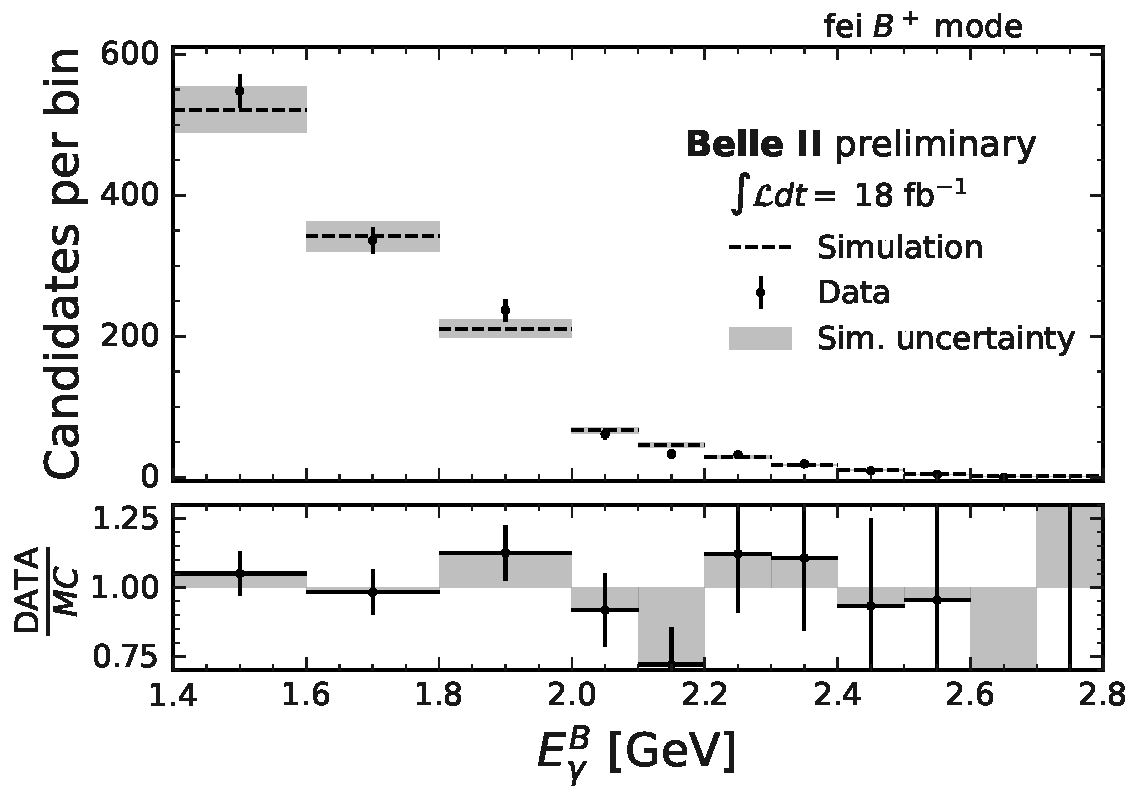
\includegraphics[width=0.31\textwidth]{figures/data_validation/Bplus_offresonance_EB.pdf}
    }
    \subcaptionbox{\label{fig:bzero_offresonance_eb}}{
        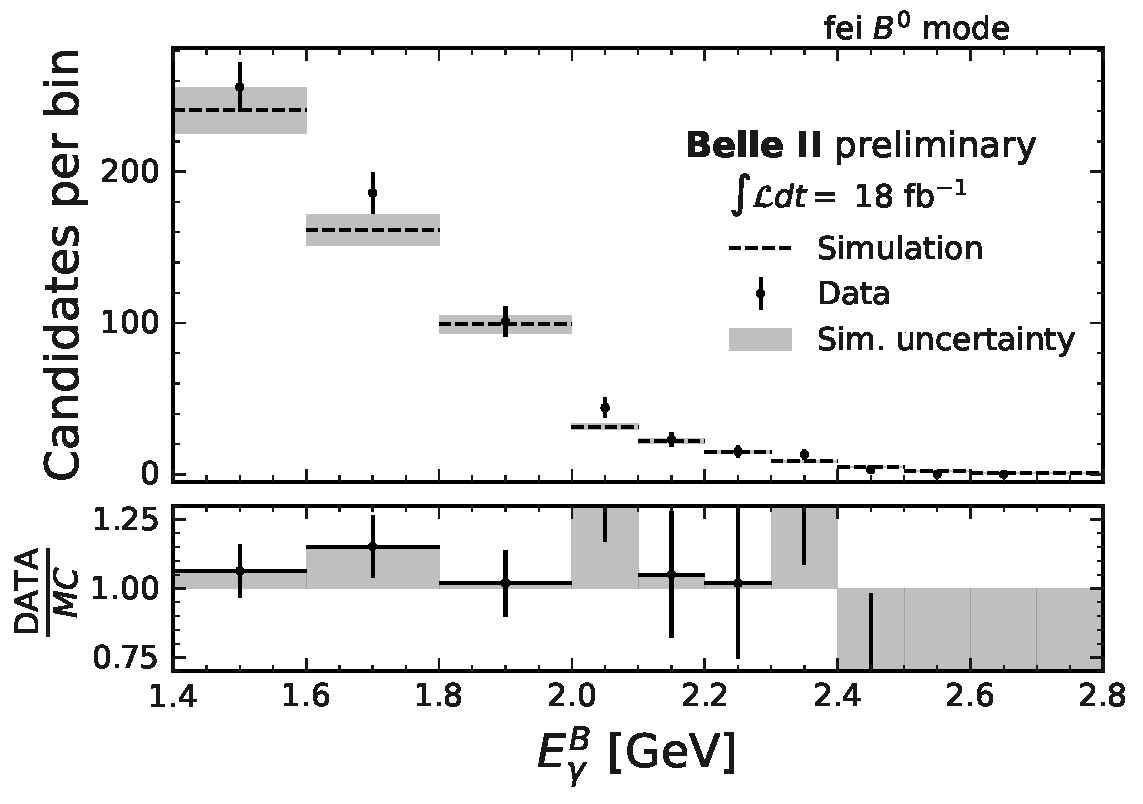
\includegraphics[width=0.31\textwidth]{figures/data_validation/Bzero_offresonance_EB.pdf}
    }
    \subcaptionbox{\label{fig:bboth_offresonance_eb}}{
        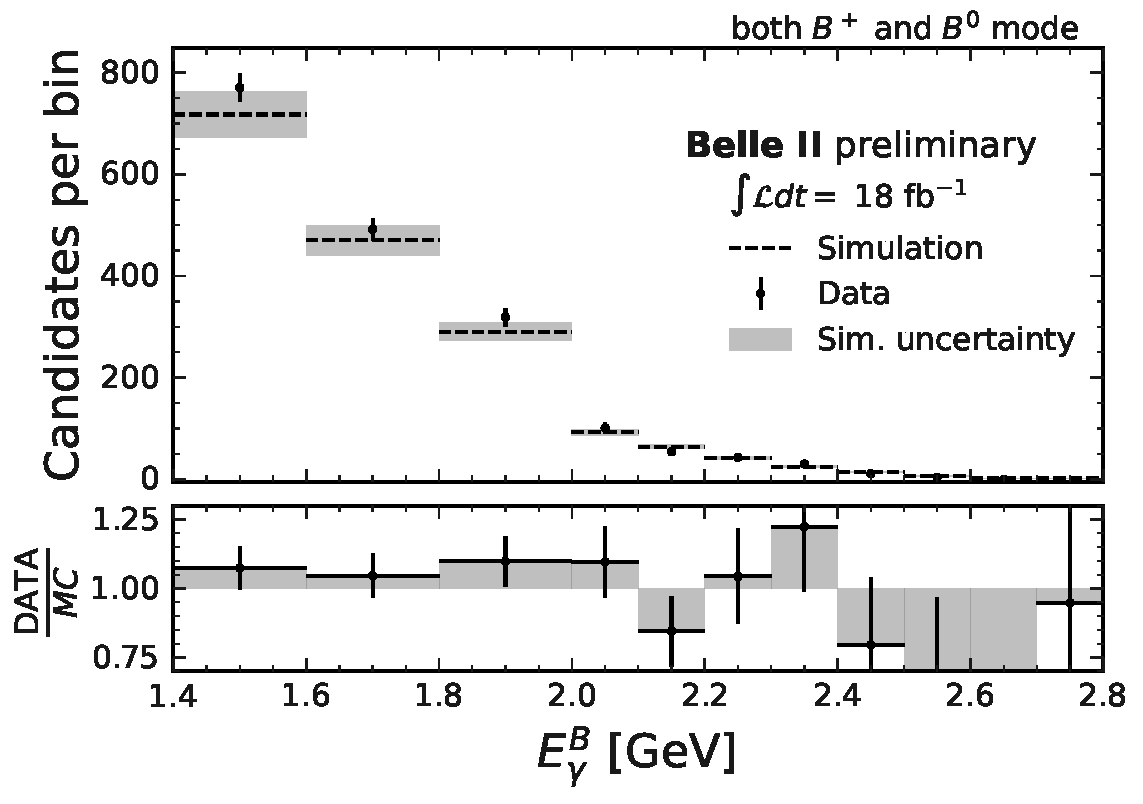
\includegraphics[width=0.31\textwidth]{figures/data_validation/Bboth_offresonance_EB.pdf}
    }
    \caption{\label{fig:offresonance_validation} Validation of the \EB distribution of \epem\ra\qqbar events.
    Excellent agreement is observed in \feiBp (\Cref{fig:bplus_offresonance_eb}, \feiBz (\Cref{fig:bzero_offresonance_eb}),
    and the combined sample (\Cref{fig:bboth_offresonance_eb}).
    The uncertainty for data contains only the statistical component.
    The simulation uncertainty contains statistical and systematic uncertainties corresponding to \Cref{tab:correction_table}.
    }
\end{figure}

Overall, the agreement of continuum data and simulation is excellent.
Due to rather low size of the off-resonance data sample and the strong continuum suppression in this analysis, the amount of statistical uncertainties are relatively large.
It is concluded, that the \EB distribution of \epem\ra\qqbar events is well-modelled in simulation and follows the expectations seen in earlier Sections.

Due to known issues with beam energy values in the off-resonance data, which affected the \Mbc calculation (but not overall validity of other values), 
the \epem\ra\qqbar off-resonance \Mbc distributions do not accurately represent the \Mbc values of continuum events.
Therefore, these samples are not used for \Mbc distribution and \Mbc fitting validation.

\subsection{Validation on \texorpdfstring{\epem\ra\qqbar}{e+e- -> qqbar} enhanced sample}\label{sec:continuum_mbc_validation}

As it was mentioned in \Cref{sec:continuum_spectrum_validation}, due to problems in \Mbc distribution, 
the dedicated \epem\ra\qqbar-only samples were not used to validate the continuum simulation.
However, an alternative validation sample is prepared, where the continuum component is enhanced.
This is achieved by inverting the \texttt{BDT~output} selection (see \Cref{sec:continuum_suppression}) thereby suppressing \BB events.
To ensure a minimal amount of \BtoXsgamma events in the sample (as the \texttt{BDT~output} is not perfectly efficient), here \piVeto and \etaVeto
are also inverted.
This creates a sample with mostly \epem\ra\qqbar events and small components of \BB events.
The inverted values are chosen as $\mathtt{BDT~output}<0.2$ and $\piVeto>0.4$ and $\etaVeto>0.4$.
The resulting \EB spectra for both \FEI modes are shown in \Cref{fig:qqbar_enhanced_eb_validation}.
\begin{figure}[htbp!]
    \subcaptionbox{\label{fig:bplus_qqbar_enhanced_eb}}{
        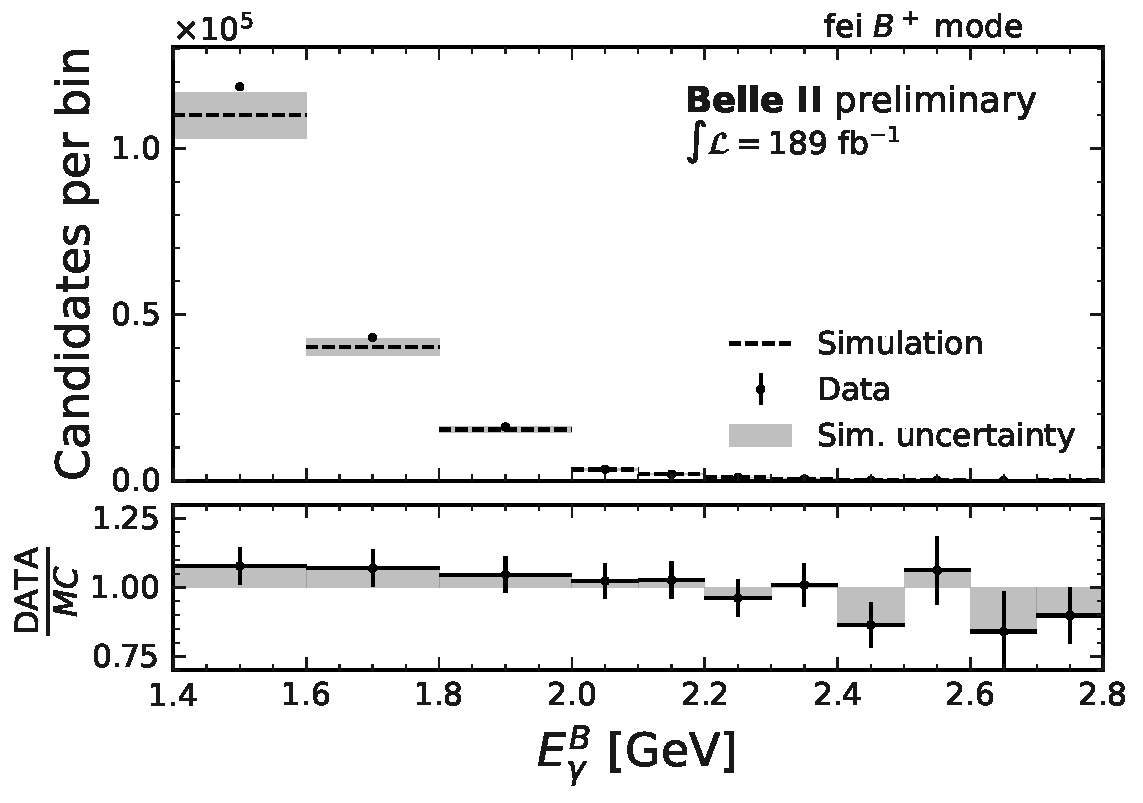
\includegraphics[width=0.31\textwidth]{figures/data_validation/Bplus_qqbar_enhanced_eb.pdf}
    }
    \subcaptionbox{\label{fig:bzero_qqbar_enhanced_eb}}{
        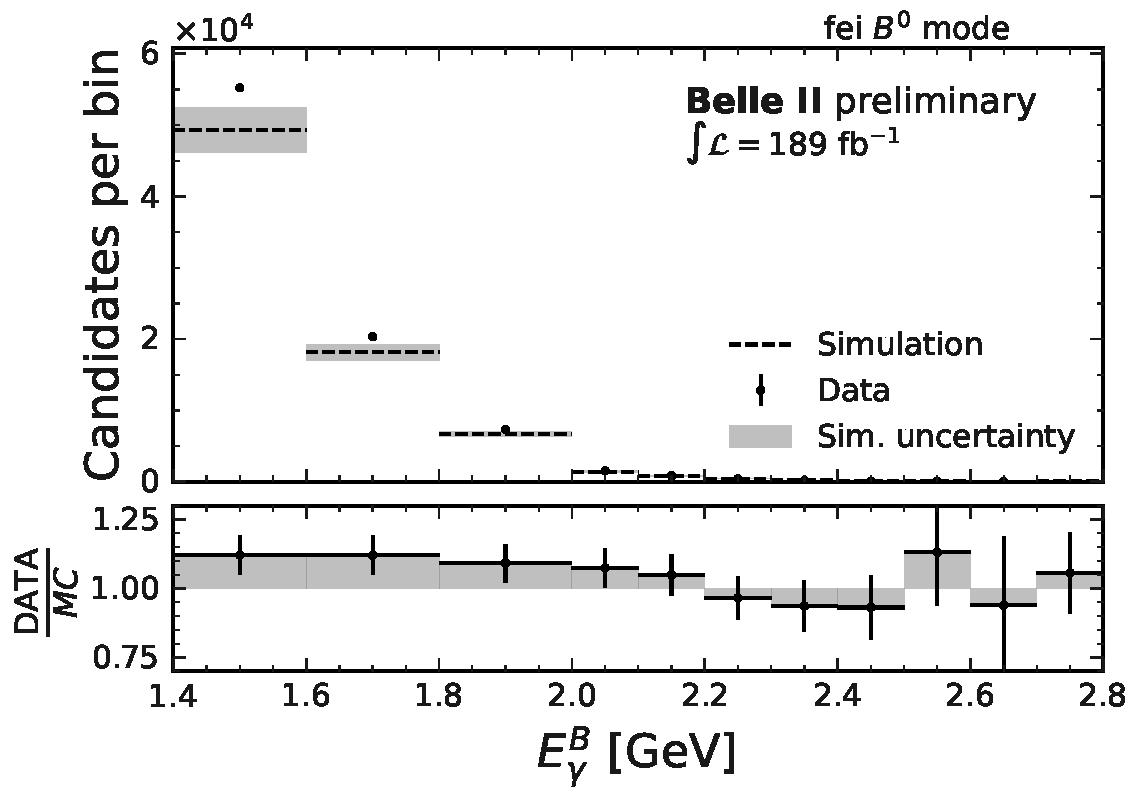
\includegraphics[width=0.31\textwidth]{figures/data_validation/Bzero_qqbar_enhanced_eb.pdf}
    }
    \subcaptionbox{\label{fig:bboth_qqbar_enhanced_eb}}{
        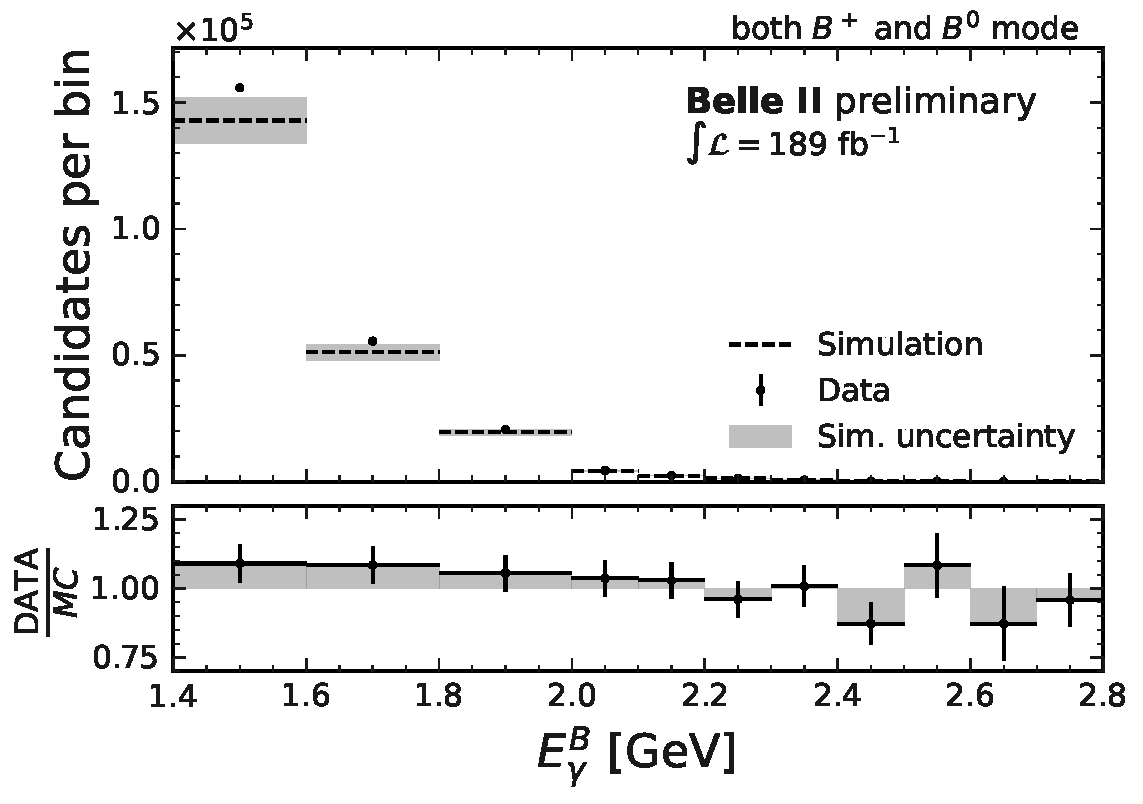
\includegraphics[width=0.31\textwidth]{figures/data_validation/Bboth_qqbar_enhanced_eb.pdf}
    }
    \caption{\label{fig:qqbar_enhanced_eb_validation} The \EB distribution of \qqbar enhanced samples (see \Cref{sec:continuum_spectrum_validation}).
    Adequate agreement is observed in \feiBp (\Cref{fig:bplus_offresonance_eb}, \feiBz (\Cref{fig:bzero_offresonance_eb}),
    and the combined sample (\Cref{fig:bboth_offresonance_eb}).
    The uncertainty for data contains only the statistical component.
    The simulation uncertainty contains statistical and systematic uncertainties corresponding to \Cref{tab:correction_table}.
    }
\end{figure}

Although the agreement is generally adequate, particularly in the signal region, although a small excess of events is observed in low-\EB region.
Similarly, the resulting \Mbc distributions are shown in \Cref{fig:qqbar_enhanced_mbc}.
A striking difference from the generally good agreement observed so far can be seen for \feiBp, \feiBz and the combined sample.
A larger amount of continuum events, particularly at low-\Mbc is present and,
moreover, the high-endpoint of the \Mbc is shifted.
The overall data-to-simulation discrepancy can be at around twenty percent.
\begin{figure}[htbp!]
    \centering
    \subcaptionbox{\label{fig:Bplus_qqbar_enhanced_mbc}}{
        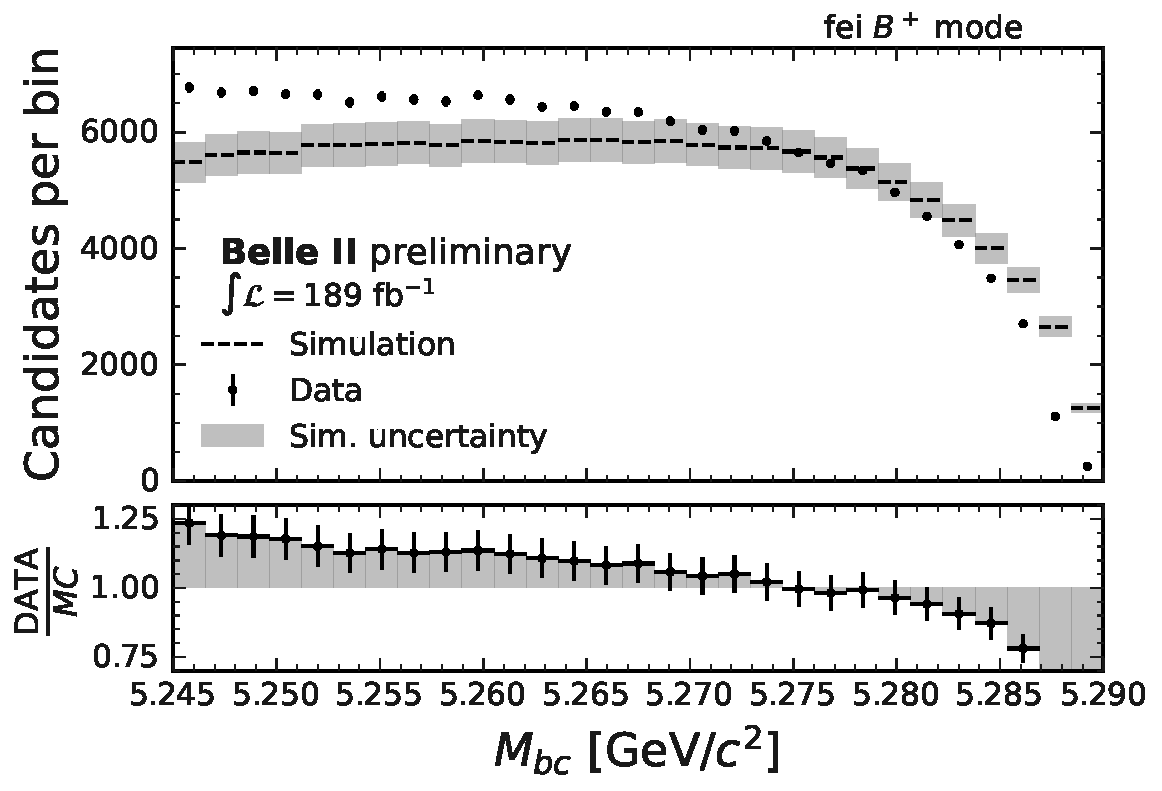
\includegraphics[width=0.31\textwidth]{figures/data_validation/Bplus_qqbar_enhanced_mbc.pdf}
    }
    \subcaptionbox{\label{fig:Bzero_qqbar_enhanced_mbc}}{
        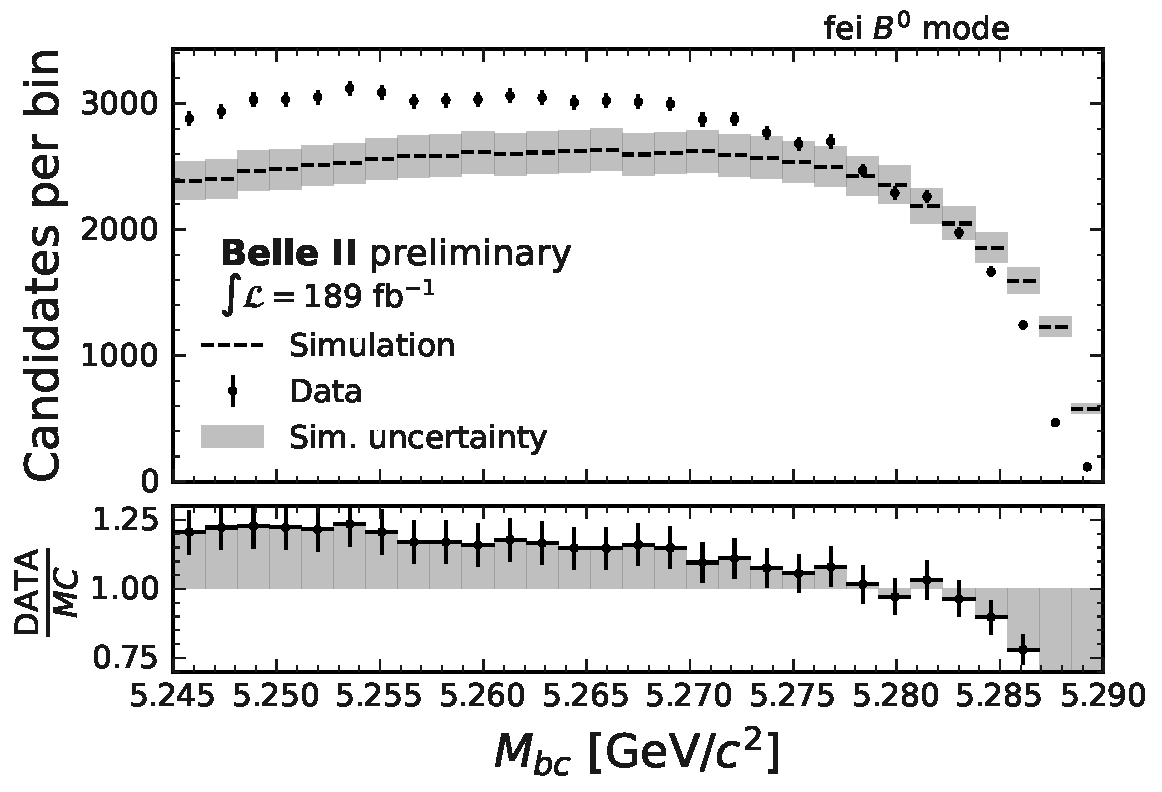
\includegraphics[width=0.31\textwidth]{figures/data_validation/Bzero_qqbar_enhanced_mbc.pdf}
    }
    \subcaptionbox{\label{fig:Bboth_qqbar_enhanced_mbc}}{
        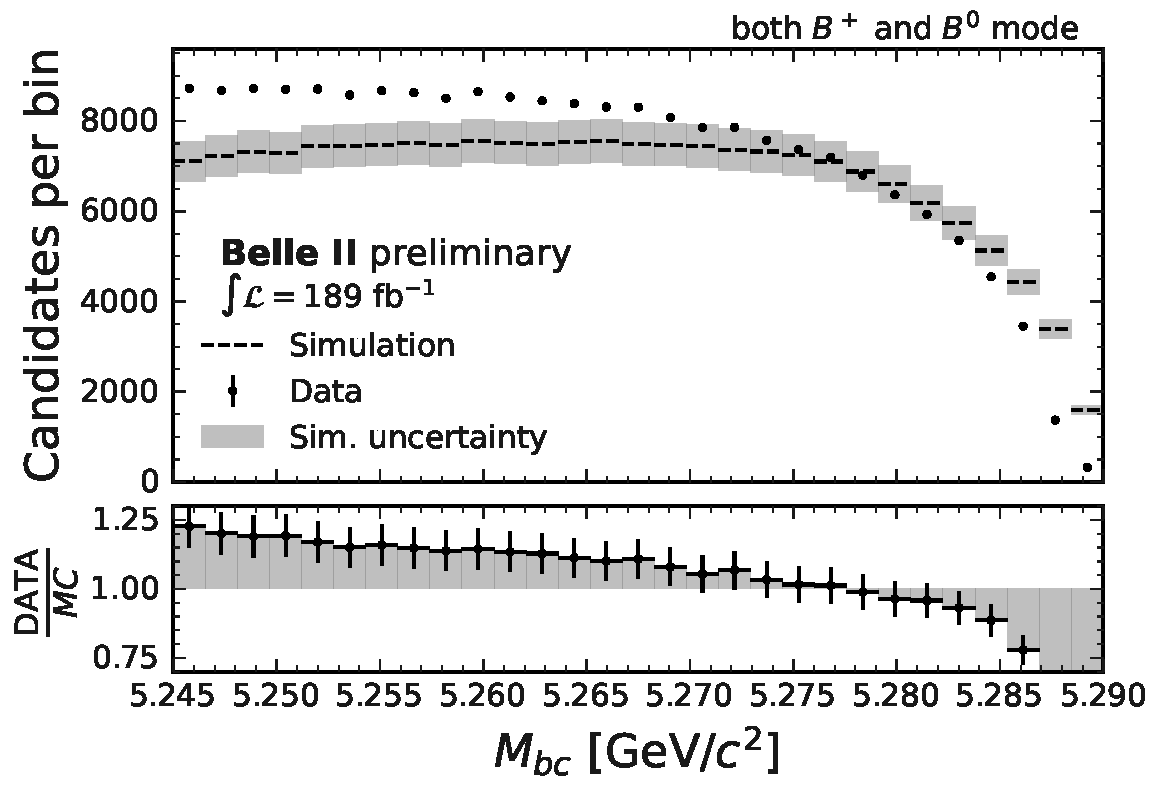
\includegraphics[width=0.31\textwidth]{figures/data_validation/Bboth_qqbar_enhanced_mbc.pdf}
    }
    \caption{\label{fig:qqbar_enhanced_mbc}
    The \Mbc distribution of \qqbar enhanced samples (see \Cref{sec:continuum_spectrum_validation}).
    Some clear differences in \feiBp (\Cref{fig:Bplus_qqbar_enhanced_mbc}), \feiBz (\Cref{fig:Bzero_qqbar_enhanced_mbc}),
    and the combined sample (\Cref{fig:Bboth_qqbar_enhanced_mbc}) can be observed.
    Particularly, it is evident that there are more continuum events at low-\Mbc, 
    and the \Mbc high-endpoint is shifted to lower values.
    These results motivate the modification of the \Mbc fitting procedure, 
    summarised in \Cref{tab:fitting_init_params_updated}.
    }
\end{figure}

These differences are understood as a result of two reasons related to the fact that data-taking period independent simulation is used in this analysis.
In normal data collection conditions, the collision energy, $\sqrt{s}$ is not perfectly stable: minute variations or drifts can occur over time.
These can be related to many reasons including intentional, such as various tests, and unintentional, such as 
The data-taking period independent simulation does not account for these changes, with a collision energy simply set to a predetermined target value.
The \Mbc endpoint is directly affected by the set $\sqrt{s}$, as seen in \Cref{eq:mbc_exclusive}, with lower values of $\sqrt{s}$ making some values of \Mbc kinematically forbidden.
On the other hand, a larger overall amount of \qqbar events is understood as a consequence of the fact that collecting the data at lower collision energies (but now lower than \FourS energy) enhances the \epem\ra\qqbar process cross-section.
Altogether, this leads to more continuum events present in the data sample than predicted by the data-taking period independent simulation.

Note that for correctly reconstruced \B mesons (i.e. good tag-\B mesons) the shift would not occur.
This is a result of the fact that $p_B^*$ (as seen in \Cref{eq:mbc_exclusive}) is directly related to the total energy of the collision.
Lower collision energies will simply lower $p_B^*$, as the resonant-like behaviour in \Mbc is driven by the \B meson mass.
Such constraints are not present for misreconstructed events, therefore shifts are expected to happen there.

Although the most robust solution is the usage of data-taking period independent simulation, at the time of preparation of this analysis such simulation was noy yet fully available at Belle II.
While future studies will be able to rely on it, in this analysis additional steps were taken to account for this.

In particular, while \Mbc is strongly affected, the \EB spectrum is still well-described.
This is a consequence of the fact that \EB and \Mbc are not strongly correlated, or more plainly, \EB does not depend as strongly on $\sqrt{s}$ as \Mbc.
Therefore, a correction is only necessary for \Mbc distribution \textit{and} only for combinatorial-\BB and continuum events.
An \textit{ad hoc} approach is developed, where the \Mbc distribution for simulated events only is shifted manually. 
The procedure is as follows:
\begin{itemize}
    \item Count the frequencies of each $\sqrt{s}$ value occurring in the Belle II on-resonance dataset.
    \item Randomly remove half of the beam energies in simulated Belle II dataset of \textit{events where no good tag-\B mesons are present}.
    \item Replace the removed beam energies with the values of the first step, based on the frequencies they occur at in the Belle~II on-resonance dataset.
\end{itemize}
The reason why only $50\%$ of energies are replaced is to minimise any potential bias that such a procedure could introduce.
Note that the replacement of $\sqrt{s}$ only affects the \Mbc calculation and not other observables which may be rely on $\sqrt{s}$ in their definition.
The result of the correction on the \Mbc distribution of the sample of both \FEI modes combined is shown in \Cref{fig:qqbar_enhanced_mbccorrected}.
\begin{figure}[htbp!]
    \centering
    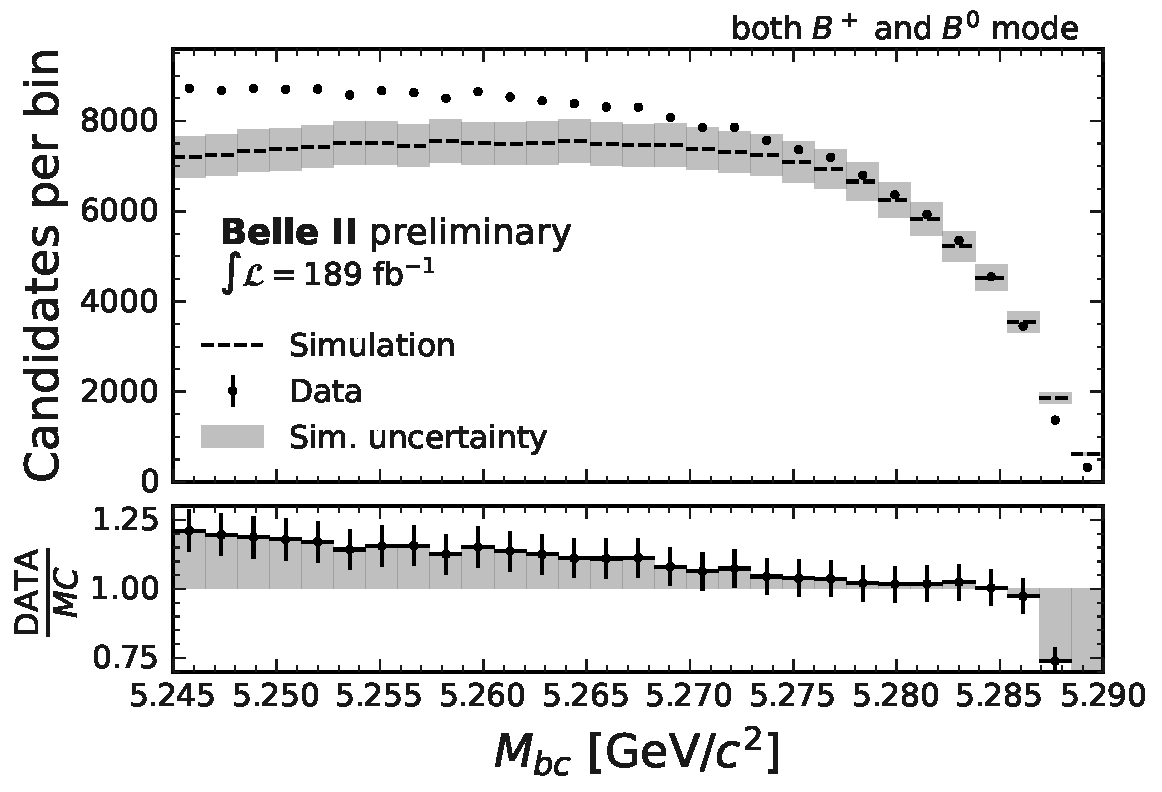
\includegraphics[width=0.45\textwidth]{figures/data_validation/Bboth_qqbar_enhanced_mbccorrected.pdf}
    \caption{\label{fig:qqbar_enhanced_mbccorrected} The \Mbc distribution of \qqbar enhanced samples (see \Cref{sec:continuum_spectrum_validation}),
    where an \Mbc correction has been applied to the simulated distribution.
    Although the correction does not perfectly correct the distributions, the signal region ($\Mbc\approx5.28~\gevcc$) is described correctly.}
\end{figure}
Although perfect correction is not achieved via this \textit{ad hoc} correction, but the peak-region is described correctly, which is evident when comparing \Cref{fig:qqbar_enhanced_mbccorrected} and \Cref{fig:qqbar_enhanced_mbc}.

A key point to discuss here is the effect the different \Mbc shape may have on the \Mbc fitter.
The differences in the tail, and the end-point are expected to not strongly affect the result, because the \Mbc fitter is prepared with shape differences and accounts for them
by estimating parameters $c$ and $m_0$ of the argus distribution, as well ass the overall $\frac{\mathcal{N}_{\mathrm{CHEB}}}{\mathcal{N}_{\mathrm{ARGUS}}}$ ratio.
However, the \Mbc fitter initial parameters in \Cref{tab:fitting_init_params} have to be updated to emphasise that a different `corrected'-\Mbc is the new fitting observable.
The \Mbc fitter is therefore updated, following the exact same procedures as \Cref{sec:fitting_setup} and the new values are given in \Cref{tab:fitting_init_params_updated}.
\begin{table}[htbp!]
    \centering
    \caption{\label{tab:fitting_init_params_updated} The summary of the fitting model used in this analysis for the \Mbc fit after updating the initial values to correspond for the correction in \Mbc distributions of background, as discussed in \Cref{sec:continuum_spectrum_validation}.
    The paramaters are initialised at the values that are listed, corresponding to the ones determined in the primary fitting steps, explained in \Cref{sec:crystal_ball_prefit,sec:chebyshev_prefit,sec:argus_prefit}, with \Mbc replaced by a `corrected'-\Mbc value.
    The values that are bolded in the table are not estimated from the final \Mbc fit, but are kept at their initialised values.
    On the other hand, all non-bolded values are estimated from the final fitter.
    The uncertainties are those estimated using the \texttt{HESSE} method.
    }
    \resizebox{1\textwidth}{!}{
    {\def\arraystretch{1.5}\tabcolsep=5pt
        \begin{tabular}{|c|c|c|c|c|c|c|c|c|c|c|c|c|c|c|}

            \hline
            \multirow{2}{*}{\EB bin} & \multicolumn{5}{|c|}{Crystal Ball} & \multicolumn{6}{c|}{Chebyshev}    & \multicolumn{3}{c|}{Argus} \\
            \cline{2-15}
                                       & $\mathcal{N}_{\mathrm{CB}}$ &$\boldsymbol{\mu}$ & $\boldsymbol{\sigma}$ & $\boldsymbol{\alpha}$ & $\mathbf{n}$ & $\mathcal{N}_{\mathrm{cheb}}$  & $\mathbf{k_1}$ & $\mathbf{k_2}$ & $\mathbf{k_3}$ & $\mathbf{k_4}$ & $\mathbf{k_5}$ & $\mathcal{N}_{\mathrm{ARGUS}}$ & $c$ & $m_0$                 \\
            \hline
            1.4 -- 1.6               & $17294\pm131$ &\multirow{11}{*}{$\mathbf{5.279}$} & \multirow{11}{*}{$\mathbf{0.003}$} & \multirow{11}{*}{$\mathbf{1.573\pm0.035}$} & \multirow{11}{*}{$\mathbf{3.561\pm0.22}$} & $70507\pm 266$& $\mathbf{-0.150\pm0.007}$ & $\mathbf{-0.382\pm0.007}$ & $\mathbf{-0.272\pm0.006}$ & $\mathbf{-0.132\pm0.006}$  & $\mathbf{-0.003\pm0.006}$  & $76798\pm277$ &  $-26.35 \pm    0.81$ & \multirow{11}{*}{$5.2897$} \\
            \cline{1-2}\cline{7-14}
            1.6 -- 1.8               & $10218\pm101$&                                      &                                        &                                   &                                  & $33666\pm183$ & $\mathbf{-0.084 \pm 0.010}$ & $\mathbf{-0.411\pm0.010}$ & $\mathbf{-0.300 \pm  0.009}$ & $\mathbf{-0.140\pm0.009}$ & $\mathbf{-0.003\pm0.009}$ & $50658\pm225$ & $-21.08 \pm 0.99$ & \\               
            \cline{1-2}\cline{7-14}
            1.8 -- 2.0               & $5947\pm77$&                                      &                                        &                                   &                                  &$16192\pm127$ & \multirow{9}{*}{$\mathbf{0.030\pm0.011}$} & \multirow{9}{*}{$\mathbf{-0.438\pm0.011}$} & \multirow{9}{*}{$\mathbf{-0.377\pm 0.009}$} & \multirow{9}{*}{$\mathbf{-0.175\pm0.010}$} & \multirow{9}{*}{$\mathbf{-0.007 \pm 0.010}$} & $31228\pm176$ & \multirow{9}{*}{$-18.64 \pm 0.93$} & \\                         
            \cline{1-2}\cline{7-7}\cline{13-13}
            2.0 -- 2.1               & $1938\pm44$&                                      &                                        &                                   &                                  & $4279\pm65$ &                 &                  &                   &                  &                    & $9983\pm100$ &                   & \\                                                                  
            \cline{1-2}\cline{7-7}\cline{13-13}
            2.1 -- 2.2               & $1246\pm35$&                                      &                                        &                                   &                                  & $2589\pm51$&                 &                  &                   &                  &                    & $6951\pm83$&                   & \\   
            \cline{1-2}\cline{7-7}\cline{13-13}
            2.2 -- 2.3               & $909\pm30$&                                      &                                        &                                   &                                  & $1581\pm40$&                &                  &                   &                  &                    &  $4470\pm67$&                  & \\   
            \cline{1-2}\cline{7-7}\cline{13-13}
            2.3 -- 2.4               & $985\pm31$&                                      &                                        &                                   &                                  & $1197\pm35$&                &                  &                   &                  &                    & $2663\pm52$&                   & \\   
            \cline{1-2}\cline{7-7}\cline{13-13}
            2.4 -- 2.5               & $1213\pm35$&                                     &                                        &                                   &                                  &$779\pm28$  &                &                  &                   &                  &                    & $1482\pm39$ &                  & \\   
            \cline{1-2}\cline{7-7}\cline{13-13}
            2.5 -- 2.6               & $626\pm25$&                                     &                                        &                                   &                                  &$310\pm18$ &                 &                  &                   &                  &                    &  $662\pm26$&                  & \\   
            \cline{1-2}\cline{7-7}\cline{13-13}
            2.6 -- 2.7               & $62\pm8$&                                     &                                        &                                   &                                  & $52\pm7$ &                &                  &                   &                  &                    & $211\pm15$ &                   & \\   
            \cline{1-2}\cline{7-7}\cline{13-13}
            2.7 -- 5.0               & $1\pm1$&                                     &                                        &                                   &                                  & $6\pm2$&                &                  &                   &                  &                    & $73\pm9$&                  & \\   
            \hline
        \end{tabular}
    }
}

\end{table}

This fitter is applied on the continuum-enhanced samples of Belle~II data used in this analysis,
and the  fitted \Mbc distributions are shown in \Cref{tab:fitting_init_params_updated}.
The figures also contain the number of good tag-\B mesons that are estimated by the fitter.
It can be seen that no statistically significant peak in \Mbc is extracted.
Therefore it can be concluded that the validation of the \Mbc fitter is successful: enough flexibility is seen
to describe the slight difference in \Mbc shapes between simulation and real data, without introducing a bias towards the extracted number of good tag-\B mesons.


\begin{figure}[htbp!]
    \centering
    \subcaptionbox{\label{fig:mbc_qqbar_ehnhanced_data_1p4}}{
        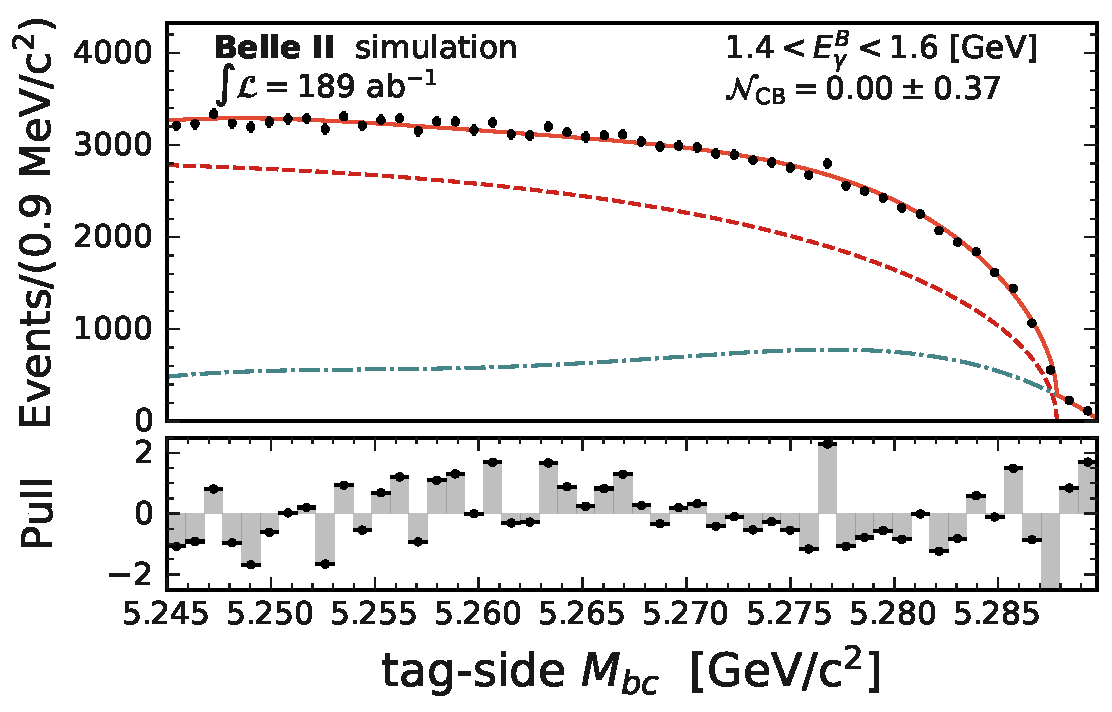
\includegraphics[width=0.3\textwidth]{figures/data_validation/qqbar_ehnaced_fits/full_MbcFit_1p4to1p6ppdf.pdf}
    }
    \subcaptionbox{\label{fig:mbc_qqbar_ehnhanced_data_1p6}}{
        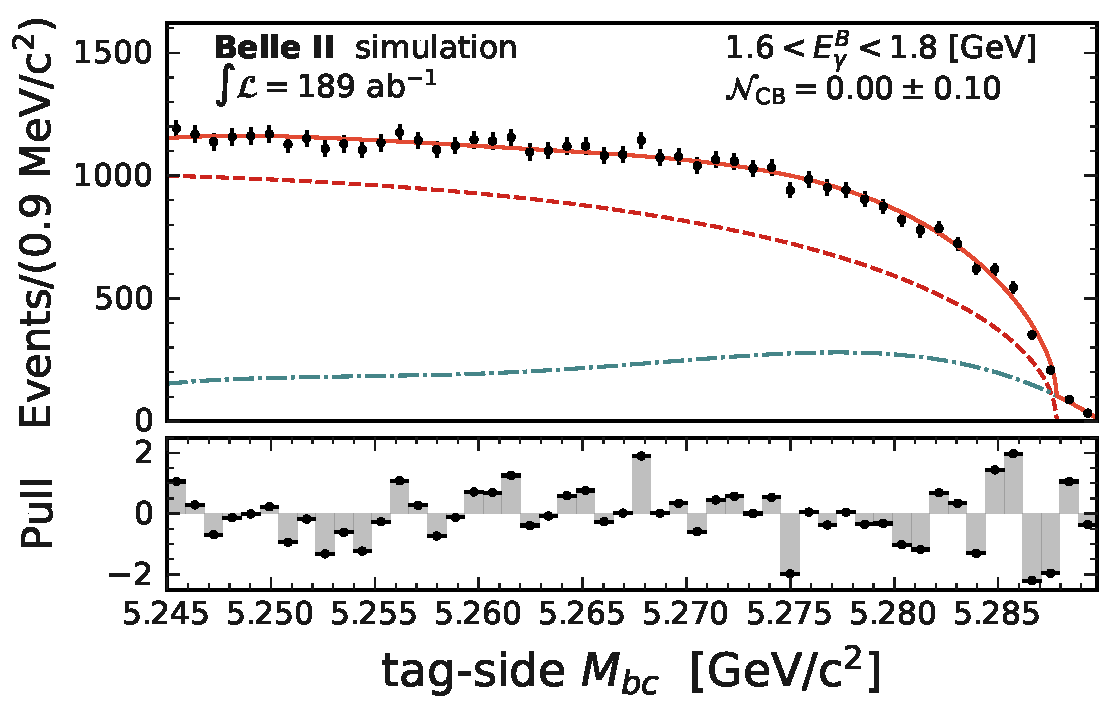
\includegraphics[width=0.3\textwidth]{figures/data_validation/qqbar_ehnaced_fits/full_MbcFit_1p6to1p8ppdf.pdf}
    }
    \subcaptionbox{\label{fig:mbc_qqbar_ehnhanced_data_1p8}}{
        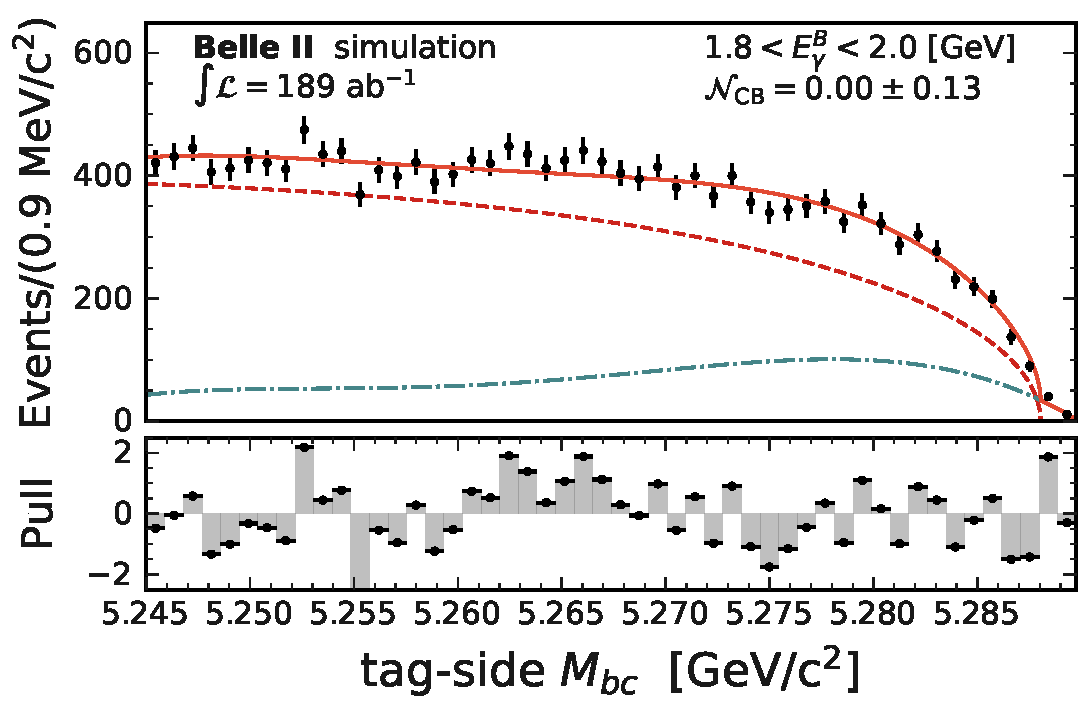
\includegraphics[width=0.3\textwidth]{figures/data_validation/qqbar_ehnaced_fits/full_MbcFit_1p8to2p0ppdf.pdf}
    }
    \subcaptionbox{\label{fig:mbc_qqbar_ehnhanced_data_2p0}}{
        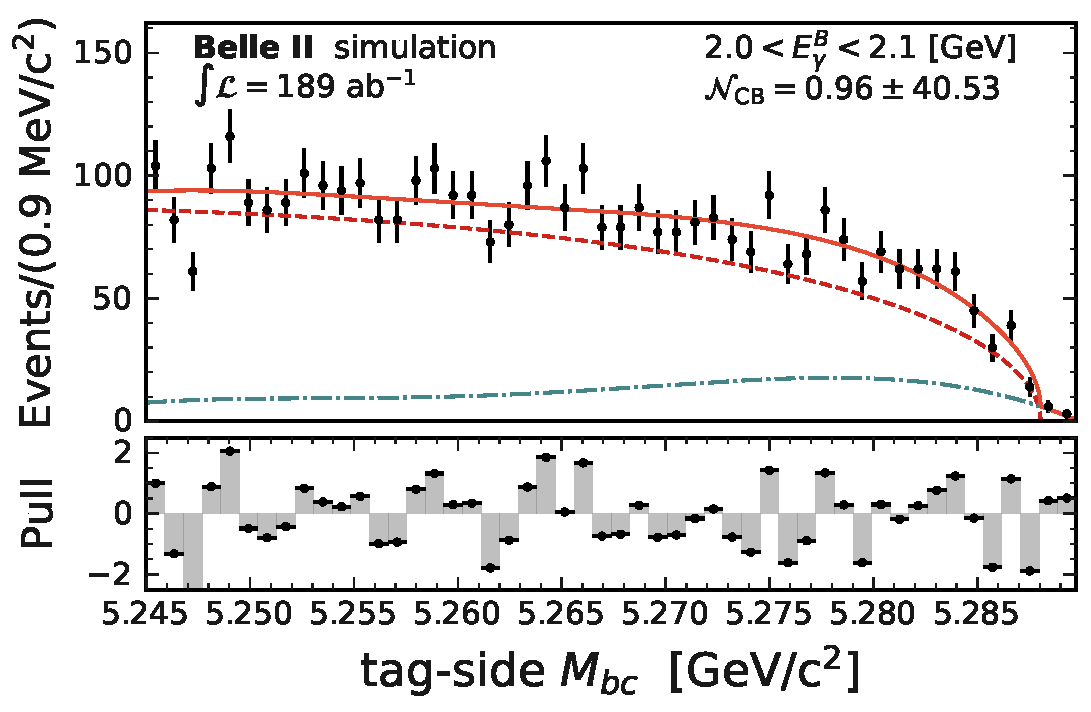
\includegraphics[width=0.3\textwidth]{figures/data_validation/qqbar_ehnaced_fits/full_MbcFit_2p0to2p1ppdf.pdf}
    }
    \subcaptionbox{\label{fig:mbc_qqbar_ehnhanced_data_2p1}}{
        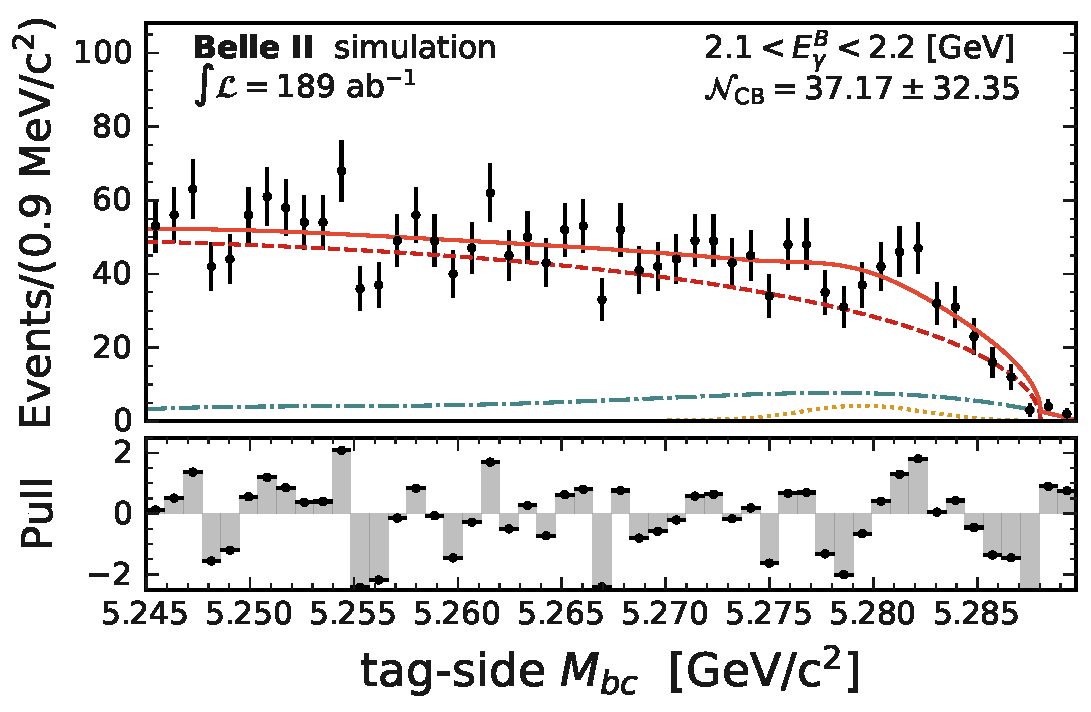
\includegraphics[width=0.3\textwidth]{figures/data_validation/qqbar_ehnaced_fits/full_MbcFit_2p1to2p2ppdf.pdf}
    }
    \subcaptionbox{\label{fig:mbc_qqbar_ehnhanced_data_2p2}}{
        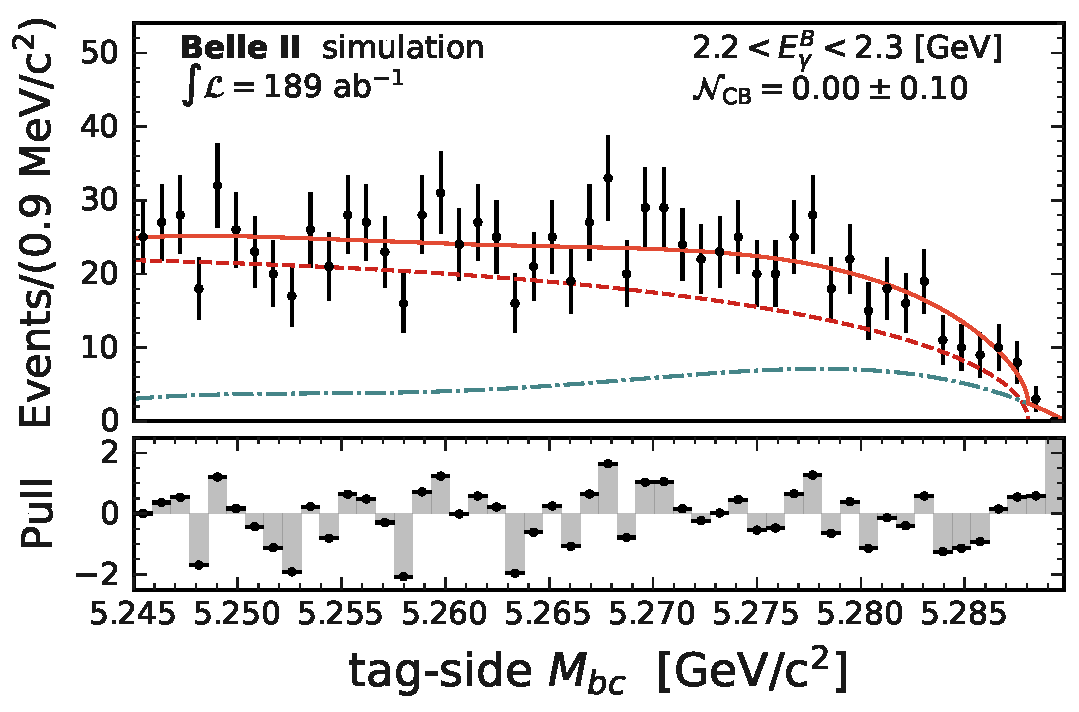
\includegraphics[width=0.3\textwidth]{figures/data_validation/qqbar_ehnaced_fits/full_MbcFit_2p2to2p3ppdf.pdf}
    }
    \subcaptionbox{\label{fig:mbc_qqbar_ehnhanced_data_2p3}}{
        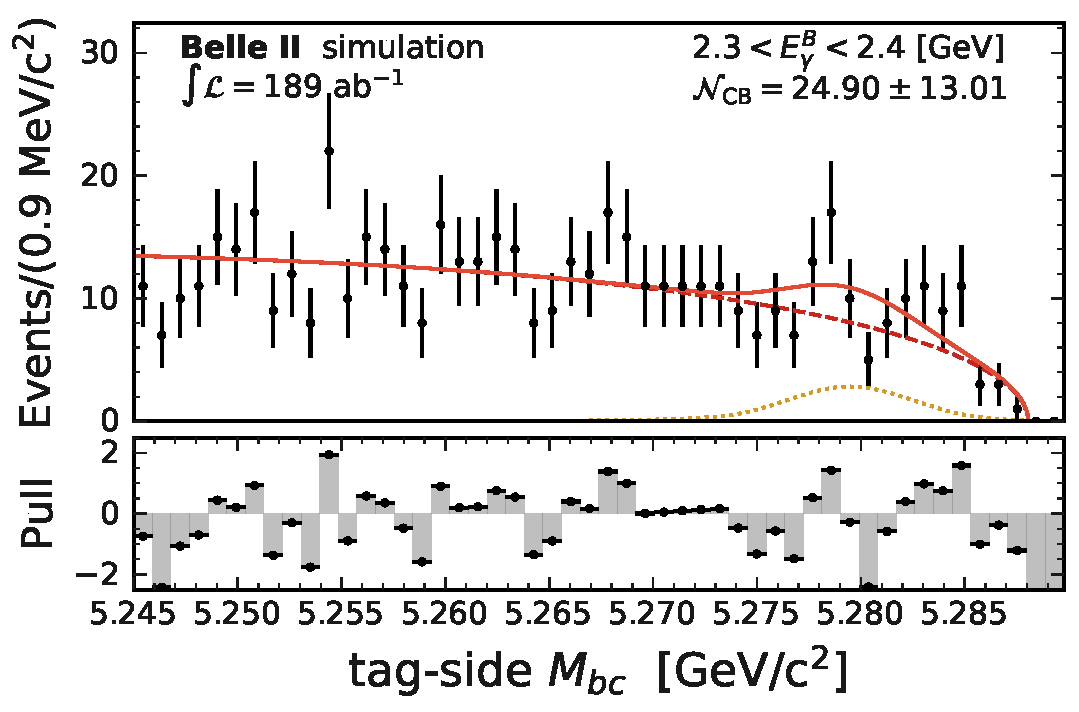
\includegraphics[width=0.3\textwidth]{figures/data_validation/qqbar_ehnaced_fits/full_MbcFit_2p3to2p4ppdf.pdf}
    }
    \subcaptionbox{\label{fig:mbc_qqbar_ehnhanced_data_2p4}}{
        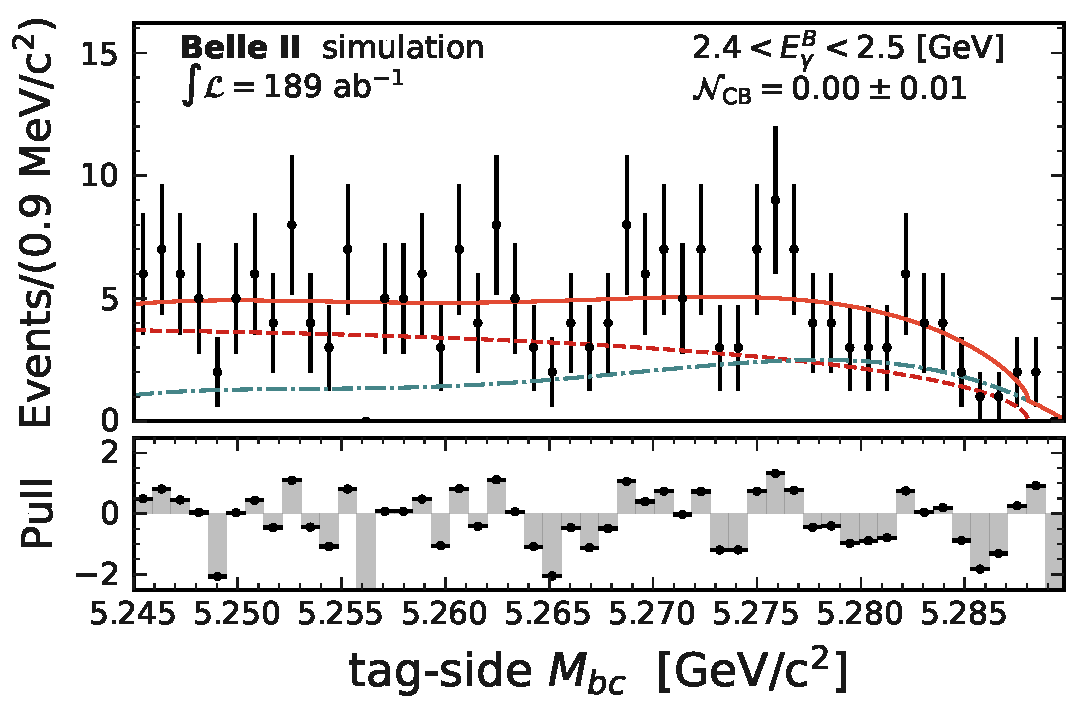
\includegraphics[width=0.3\textwidth]{figures/data_validation/qqbar_ehnaced_fits/full_MbcFit_2p4to2p5ppdf.pdf}
    }
    \subcaptionbox{\label{fig:mbc_qqbar_ehnhanced_data_2p5}}{
        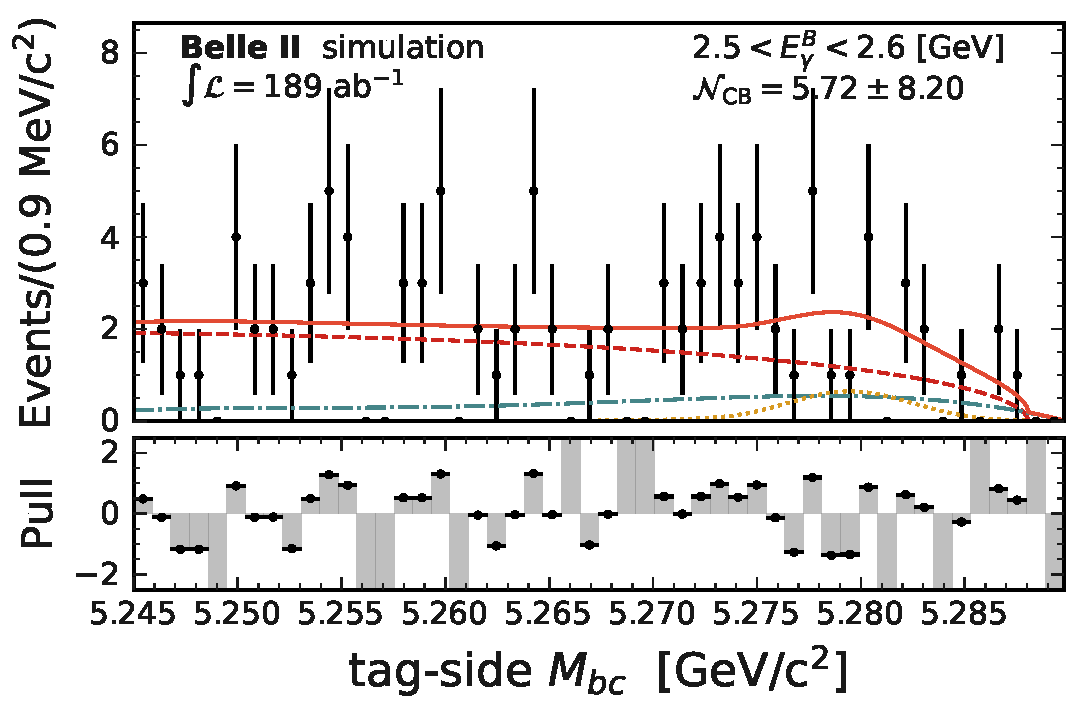
\includegraphics[width=0.3\textwidth]{figures/data_validation/qqbar_ehnaced_fits/full_MbcFit_2p5to2p6ppdf.pdf}
    }
    \subcaptionbox{\label{fig:mbc_qqbar_ehnhanced_data_2p6}}{
        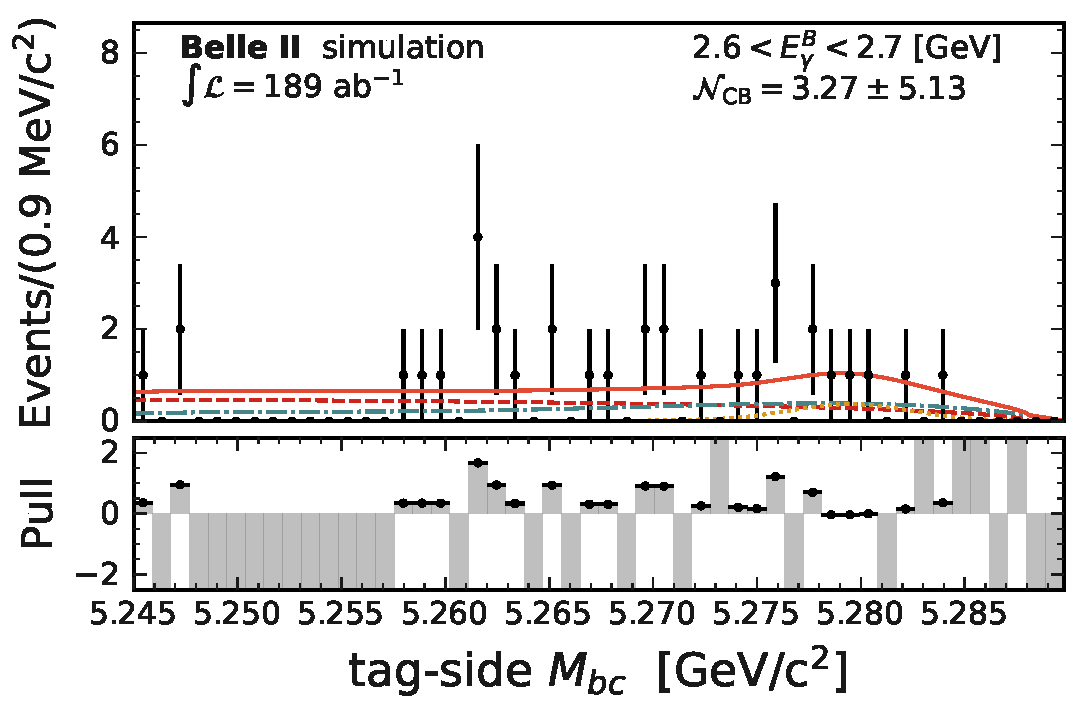
\includegraphics[width=0.3\textwidth]{figures/data_validation/qqbar_ehnaced_fits/full_MbcFit_2p6to2p7ppdf.pdf}
    }
    \subcaptionbox{\label{fig:mbc_qqbar_ehnhanced_data_2p7}}{
        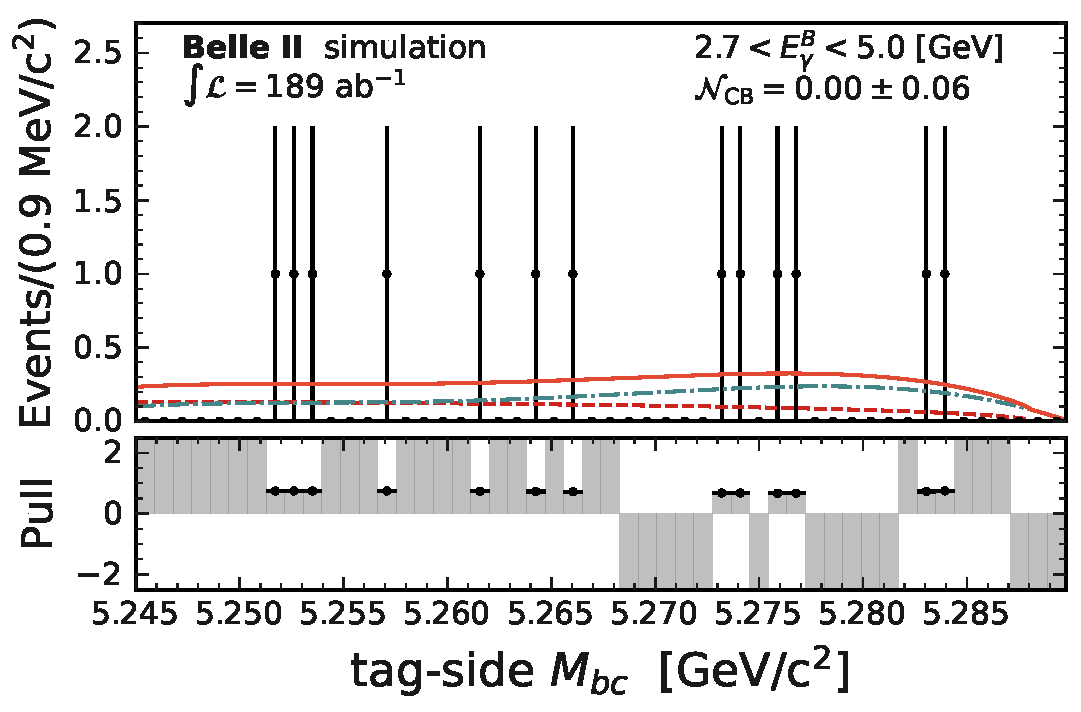
\includegraphics[width=0.3\textwidth]{figures/data_validation/qqbar_ehnaced_fits/full_MbcFit_2p7to5p0ppdf.pdf}
    }
    \caption{\label{fig:mbc_qqbar_ehnhanced_fits}The fits on Belle II dataset corresponding to 189~\invfb with selection that enhances \epem\ra\qqbar events, as discussed in \Cref{sec:continuum_spectrum_validation}.
    The fitting model from \Cref{tab:fitting_init_params_updated} is used, which is defined on the `corrected'-\Mbc to account for variations $\sqrt{s}$ in Belle II data.
    Good description of the \Mbc distributions can be seen throughout the \EB bins.
    As the continuum component in each \EB bin is enhanced, no good tag-\B mesons are expected and indeed - no statistically significant peak is extracted from the results.
    }
\end{figure}

\subsection{Validation on \texorpdfstring{\BB}{BB}-background enhanced sample}\label{sec:bb_background_validation}

In the last Section, the validation on a sample with \epem\ra\qqbar events was performed.
Another important validation given the background subtraction step (\Cref{sec:background_subtraction}),
is the \BB background decription in simulated data.

Firstly, a \BB-background enhanced sample is prepared.
This is done in almost the same manner as \Cref{sec:continuum_mbc_validation}, except with the continuum suppression requirement unchanged from the optimal selection.
In this case, only the \piVeto and \etaVeto selections are inverted.
The selections are chosen as $\piVeto>0.6$ and $\etaVeto>0.6$, as these selection ensure that the signal-to-background ratio is less than 0.1\%.
As the selections are inverted, so must the corrections that account for them be modified (\Cref{tab:correction_table}).
In particular, the corresponding corrections for the \piVeto and \etaVeto are transformed as follows:
\begin{equation}\label{eq:correction_transform}
    \mathrm{Corr}_{>0.x} = \frac{1}{\mathrm{Corr_{<0.x}}}; \quad \sigma(\mathrm{Corr}_{>0.x}) =  \frac{1}{\mathrm{Corr_{<0.x}}^2} \times \sigma(\mathrm{Corr}_{<0.x}).
\end{equation}

The \EB distribution of the \BB-enhanced sample is shown in \Cref{fig:bbbar_enhanced_eb}.
Overall, the distributions show excellent agreement between data and simulation.
The previously seen discrepancy in normalisation (see \Cref{fig:qqbar_enhanced_eb_validation}) is no longer apparent.
This can be interpreted based on the fact that here \epem\ra\qqbar events are strongly suppressed, namely 
by the requirements of \texttt{BDT~output}.
\begin{figure}[htbp!]
    \centering
    \subcaptionbox{\label{fig:Bplus_bbbar_enhanced_eb}}{
        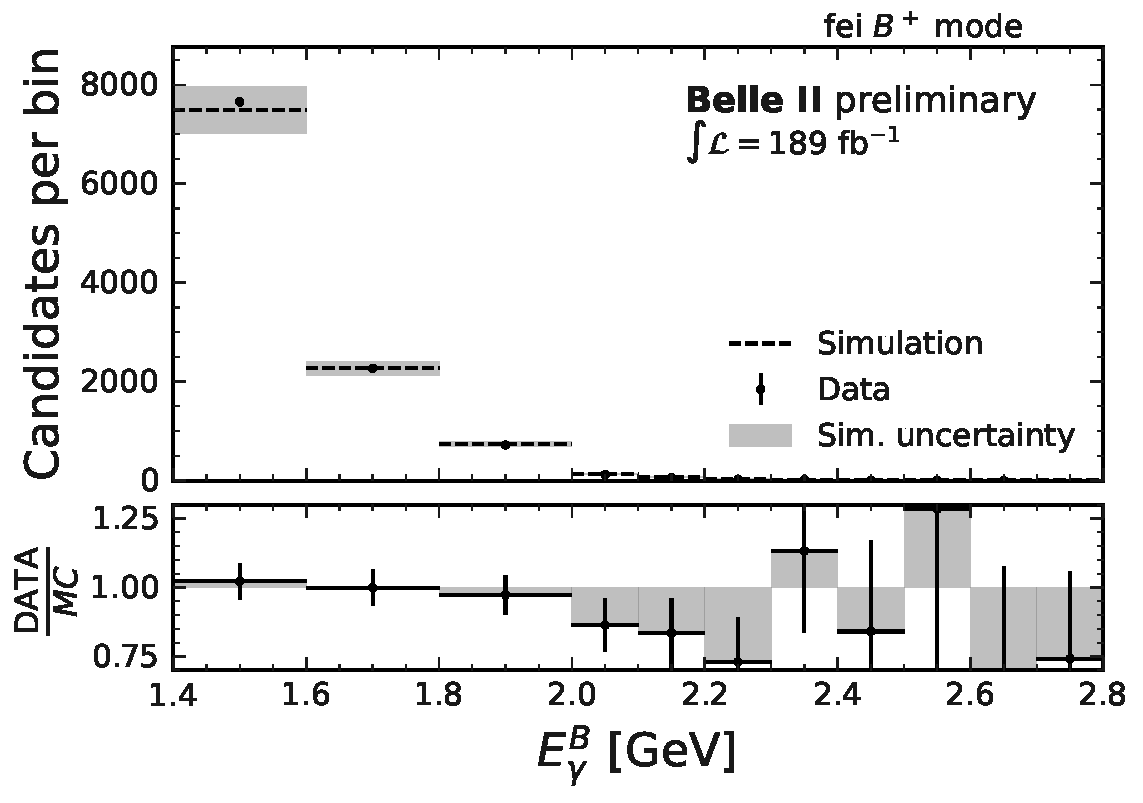
\includegraphics[width=0.3\textwidth]{figures/data_validation/Bplus_bbbar_enhanced_eb.pdf}
    }
    \subcaptionbox{\label{fig:Bzero_bbbar_enhanced_eb}}{
        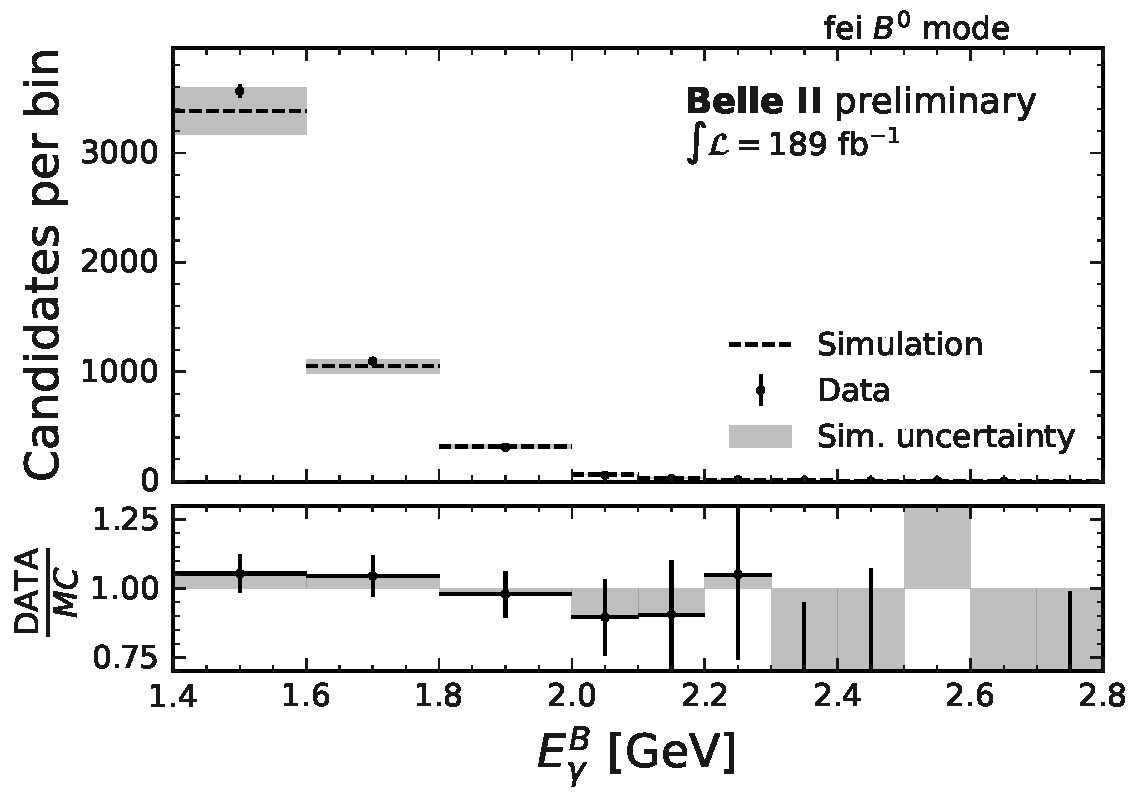
\includegraphics[width=0.3\textwidth]{figures/data_validation/Bzero_bbbar_enhanced_eb.pdf}
    }
    \subcaptionbox{\label{fig:Bboth_bbbar_enhanced_eb}}{
        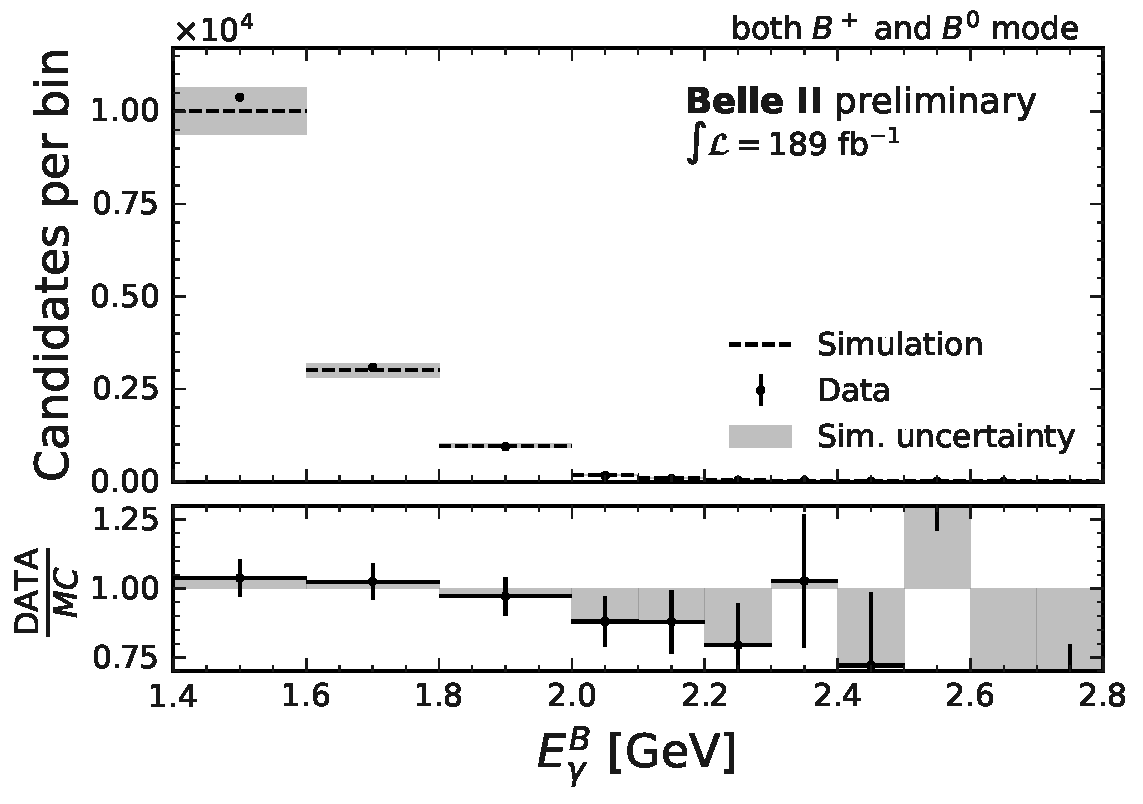
\includegraphics[width=0.3\textwidth]{figures/data_validation/Bboth_bbbar_enhanced_eb.pdf}
    }
    \caption{\label{fig:bbbar_enhanced_eb} The \EB distribution of \BB-background enhanced samples (see \Cref{sec:bb_background_validation}).
    Compared to \Cref{fig:bboth_offresonance_eb}, it is clear that the \BB background drops off faster with increasing \EB than \epem\ra\qqbar.
    Overall, the data-simulation agreement is excellent and this is attributed to the fact that continuum events, which were accredited to causing a discrepancy in \Cref{sec:continuum_spectrum_validation}, are highly suppressed in the \BB-background enhanced sample.
    }
\end{figure}

Following the observations in \Cref{sec:continuum_mbc_validation}, similar modifications to \Mbc are necessary here, too.
The corrected-\Mbc distribution is shown in \Cref{fig:bbbar_enhanced_mbccorrected}.
The results are shown for the combined \feiBp and \feiBz sample only, although the individual \FEI modes also show similar results.
In particular, one can see that the agreement between data and simulation is closer than what was observed in \Cref{sec:continuum_mbc_validation}.
This goes in line with the previous statements that \epem\ra\qqbar modelling was related to the discrepancies observed so far, which are not strongly pronounced here due to their suppression.
Observing the pull distribution in \Cref{fig:bbbar_enhanced_mbccorrected} it is clear that, generally, fewer events seem to be present in the peak region and more in the tail region.
Again, this is in line with the expectation: the variations of $\sqrt{s}$ in real data modify the \BB-production and \epem\ra\qqbar cross-sections.
\begin{figure}[htbp!]
    \centering
    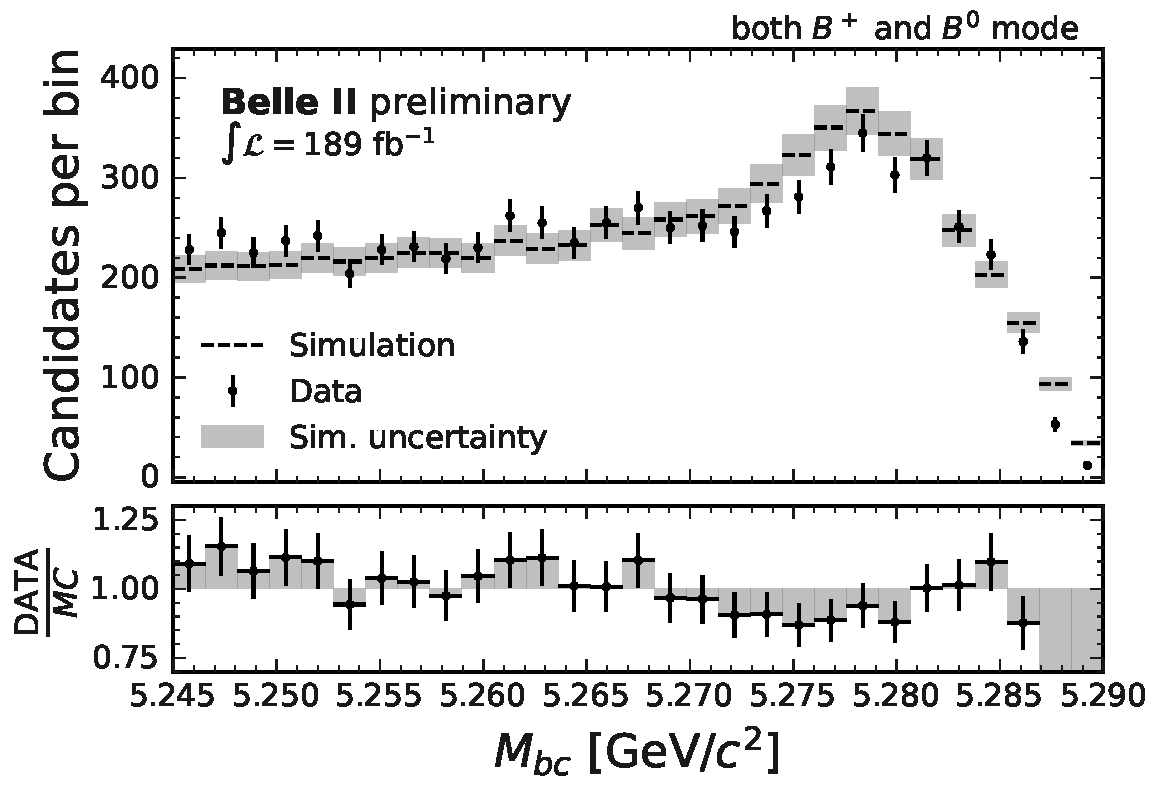
\includegraphics[width=0.45\textwidth]{figures/data_validation/Bboth_bbbar_enhanced_mbccorrected.pdf}
    \caption{\label{fig:bbbar_enhanced_mbccorrected} The \Mbc distribution of \BB-background enhanced samples (see \Cref{sec:bb_background_validation}),
    where an \Mbc correction has been applied to the simulated distribution.
    Only the \feiBp and \feiBz combined sample is shown, but the individual ones show similar results.
    Due to a lower number of \epem\ra\qqbar events, the low-\Mbc region disagreement is less pronounced than in \Cref{fig:qqbar_enhanced_mbccorrected}.
    }
\end{figure}

Finally, a fit of the \BB-enhanced performed of the \Mbc distributions, according to the modified \Mbc fitter model in \Cref{tab:fitting_init_params_updated}.
Unlike in \Cref{fig:mbc_qqbar_ehnhanced_fits}, the number of expected-\BB events is no longer expected to be negligible.
Therefore, this validation serves as a test of fit-bias and background-subtraction procedure.
The fits on Belle II simulation are shown in \Cref{fig:mbc_bbar_ehnhanced_fits_mc}, whereas the fits on Belle II data \Cref{fig:mbc_bbar_ehnhanced_fits_data}.
The figures also shown the extracted good tag-\B meson counts as normalisations of the Crystall Ball \PDF, $\mathcal{N}_{\mathrm{CB}}$.
\begin{figure}[htbp!]
    \centering
    \subcaptionbox{\label{fig:mbc_bbar_ehnhanced_mc_1p4}}{
        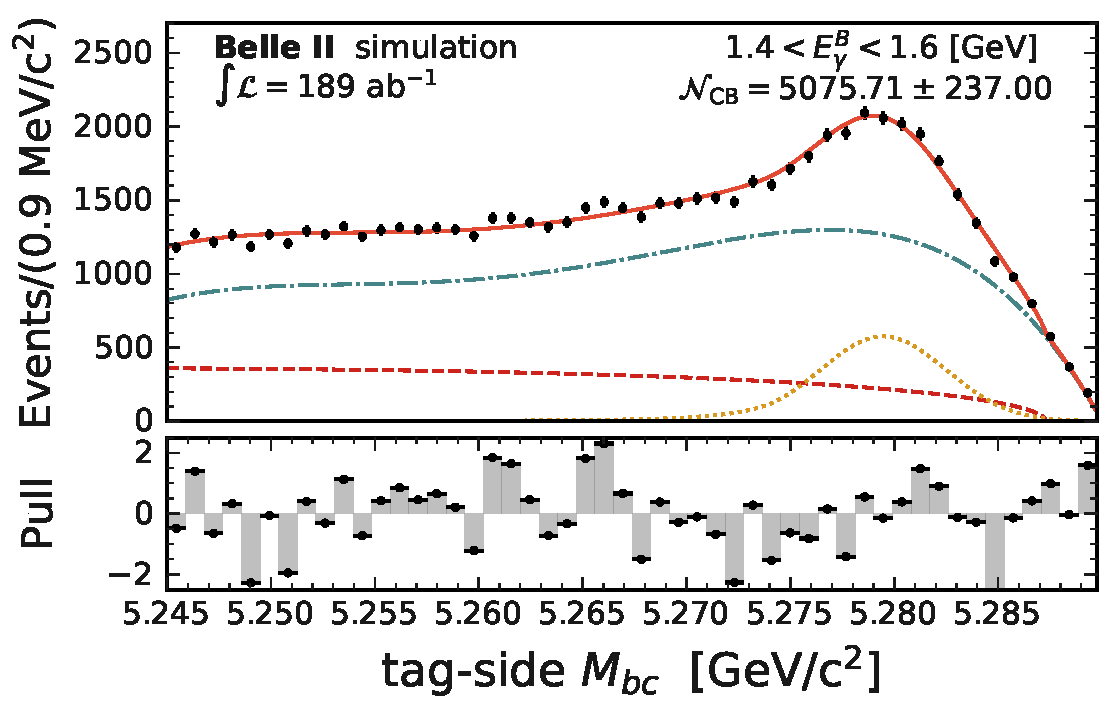
\includegraphics[width=0.3\textwidth]{figures/data_validation/bbbar_enhanced_fits/MC_MbcFit_1p4to1p6ppdf.pdf}
    }
    \subcaptionbox{\label{fig:mbc_bbar_ehnhanced_mc_1p6}}{
        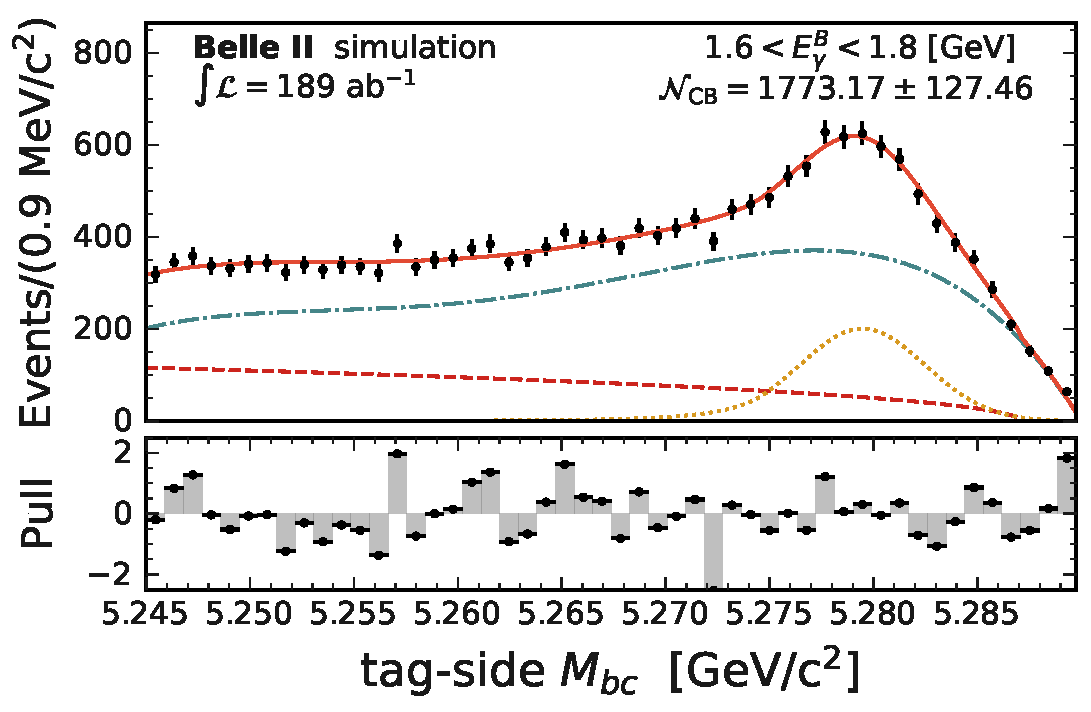
\includegraphics[width=0.3\textwidth]{figures/data_validation/bbbar_enhanced_fits/MC_MbcFit_1p6to1p8ppdf.pdf}
    }
    \subcaptionbox{\label{fig:mbc_bbar_ehnhanced_mc_1p8}}{
        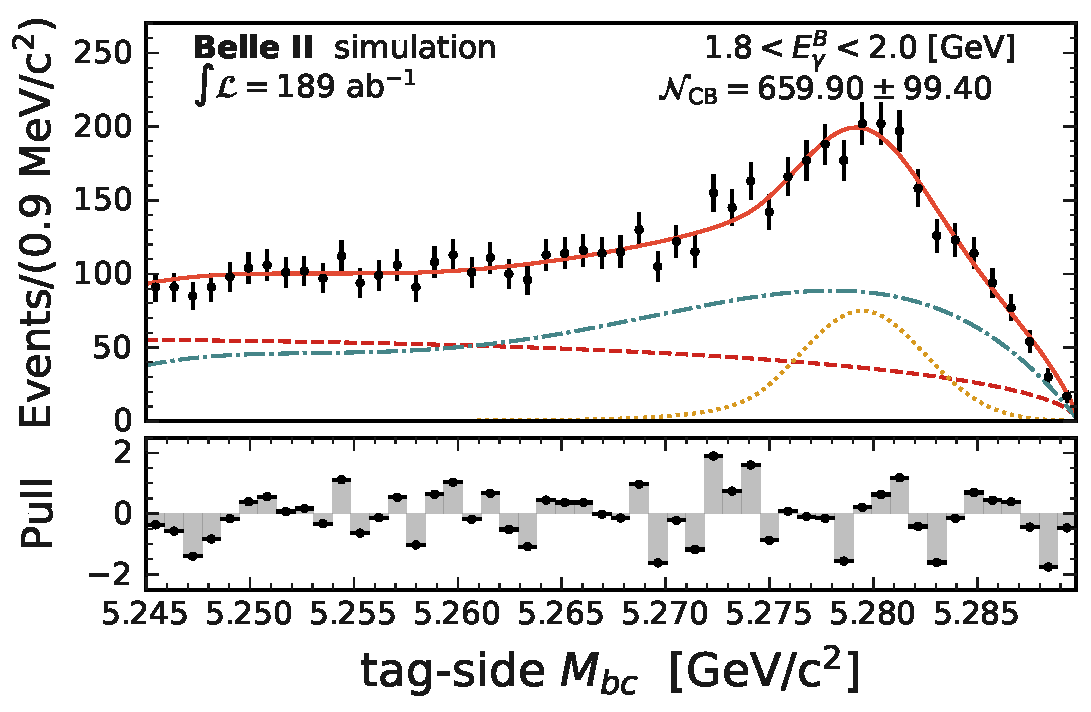
\includegraphics[width=0.3\textwidth]{figures/data_validation/bbbar_enhanced_fits/MC_MbcFit_1p8to2p0ppdf.pdf}
    }
    \subcaptionbox{\label{fig:mbc_bbar_ehnhanced_mc_2p0}}{
        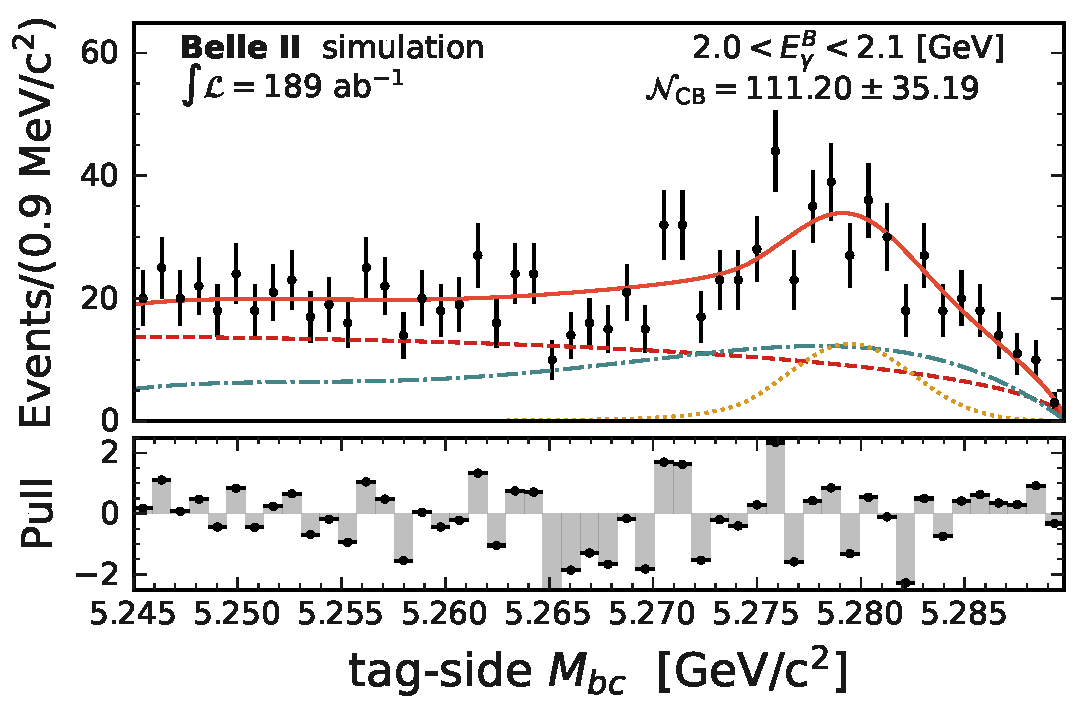
\includegraphics[width=0.3\textwidth]{figures/data_validation/bbbar_enhanced_fits/MC_MbcFit_2p0to2p1ppdf.pdf}
    }
    \subcaptionbox{\label{fig:mbc_bbar_ehnhanced_mc_2p1}}{
        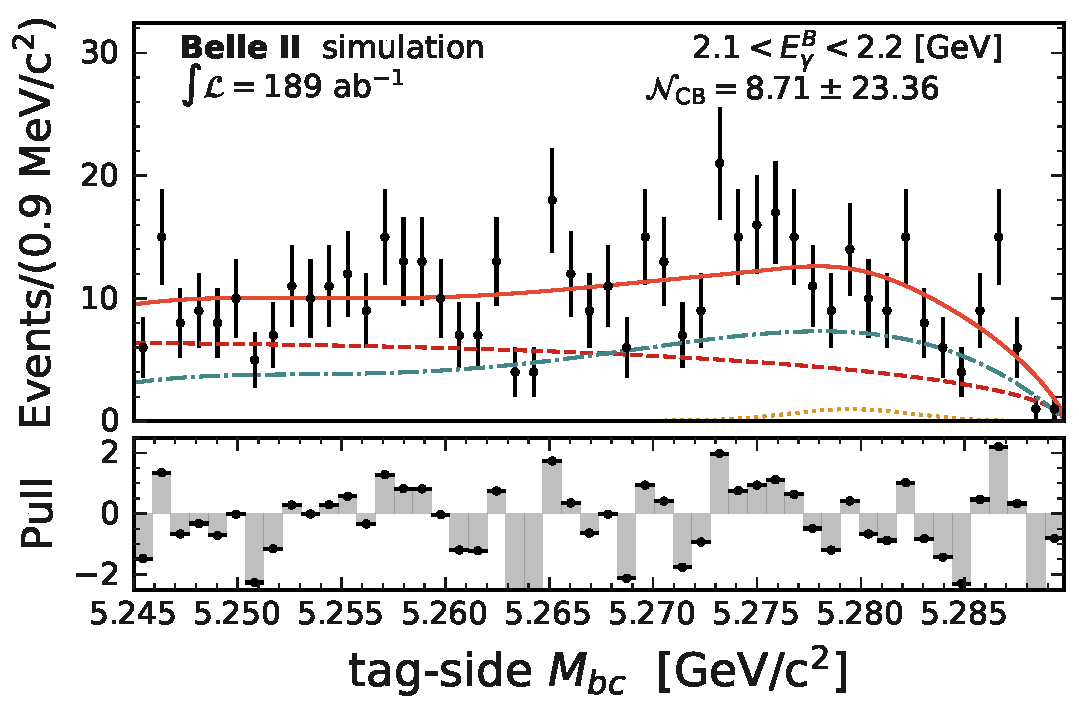
\includegraphics[width=0.3\textwidth]{figures/data_validation/bbbar_enhanced_fits/MC_MbcFit_2p1to2p2ppdf.pdf}
    }
    \subcaptionbox{\label{fig:mbc_bbar_ehnhanced_mc_2p2}}{
        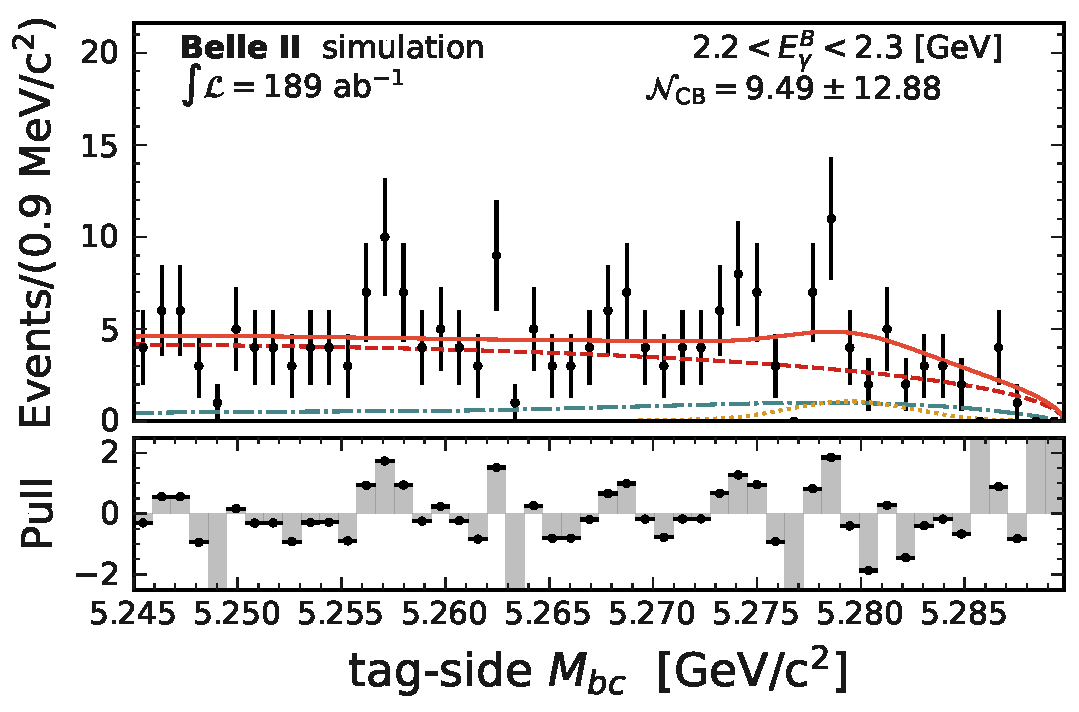
\includegraphics[width=0.3\textwidth]{figures/data_validation/bbbar_enhanced_fits/MC_MbcFit_2p2to2p3ppdf.pdf}
    }
    \subcaptionbox{\label{fig:mbc_bbar_ehnhanced_mc_2p3}}{
        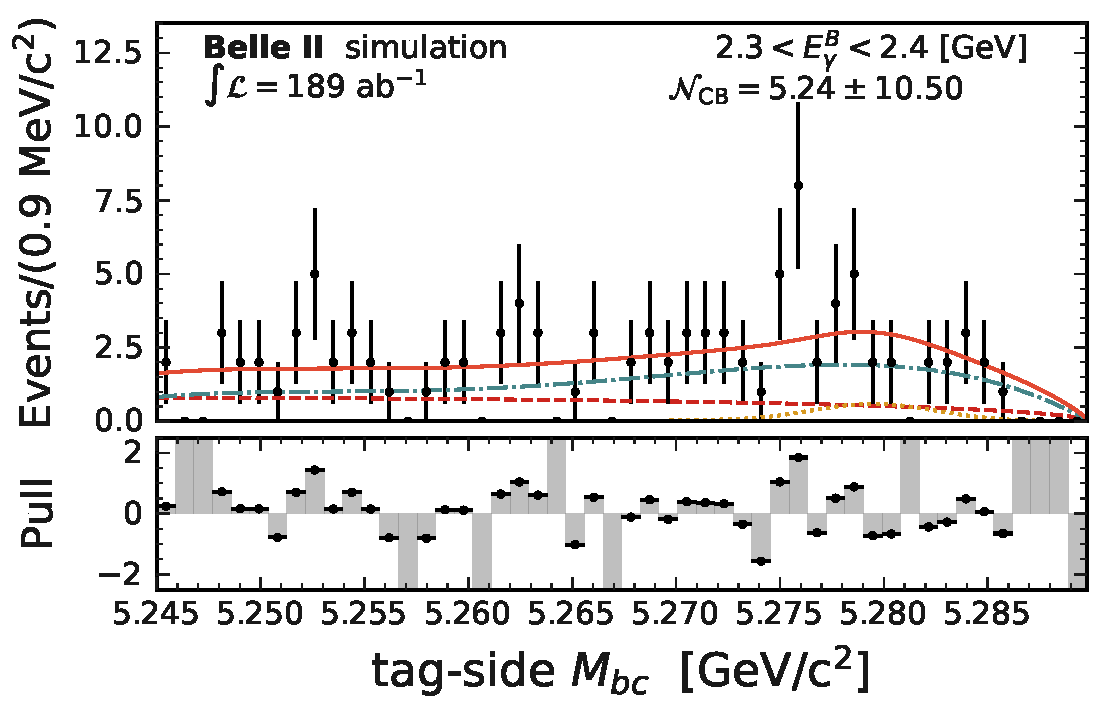
\includegraphics[width=0.3\textwidth]{figures/data_validation/bbbar_enhanced_fits/MC_MbcFit_2p3to2p4ppdf.pdf}
    }
    \subcaptionbox{\label{fig:mbc_bbar_ehnhanced_mc_2p4}}{
        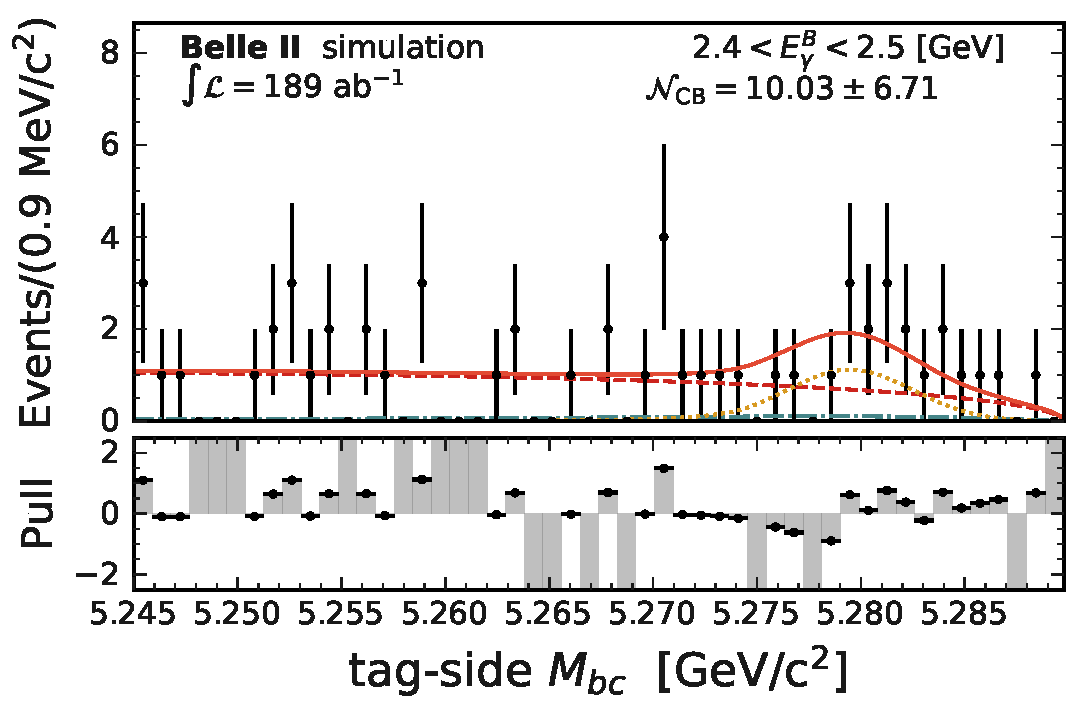
\includegraphics[width=0.3\textwidth]{figures/data_validation/bbbar_enhanced_fits/MC_MbcFit_2p4to2p5ppdf.pdf}
    }
    \subcaptionbox{\label{fig:mbc_bbar_ehnhanced_mc_2p5}}{
        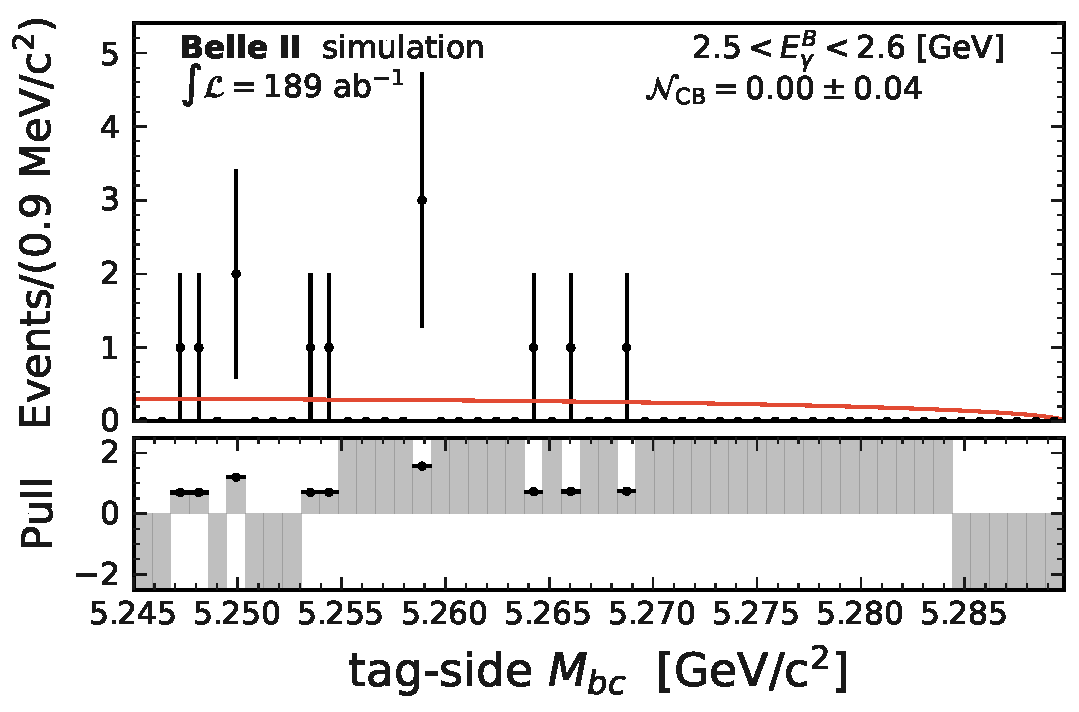
\includegraphics[width=0.3\textwidth]{figures/data_validation/bbbar_enhanced_fits/MC_MbcFit_2p5to2p6ppdf.pdf}
    }
    \subcaptionbox{\label{fig:mbc_bbar_ehnhanced_mc_2p6}}{
        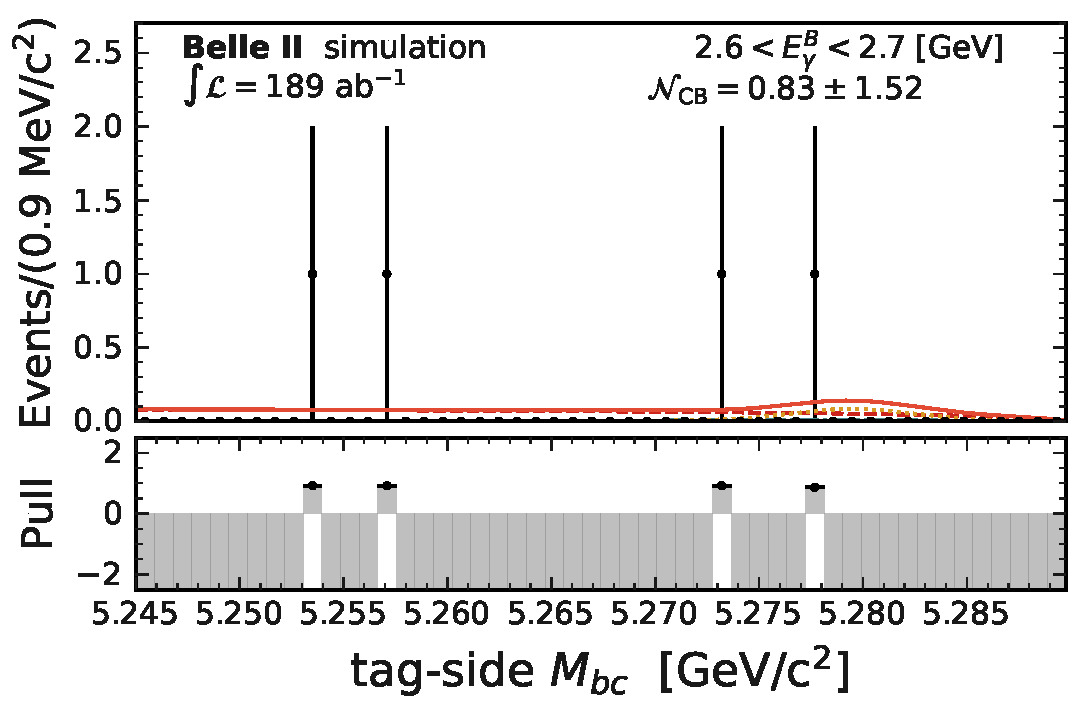
\includegraphics[width=0.3\textwidth]{figures/data_validation/bbbar_enhanced_fits/MC_MbcFit_2p6to2p7ppdf.pdf}
    }
    \subcaptionbox{\label{fig:mbc_bbar_ehnhanced_mc_2p7}}{
        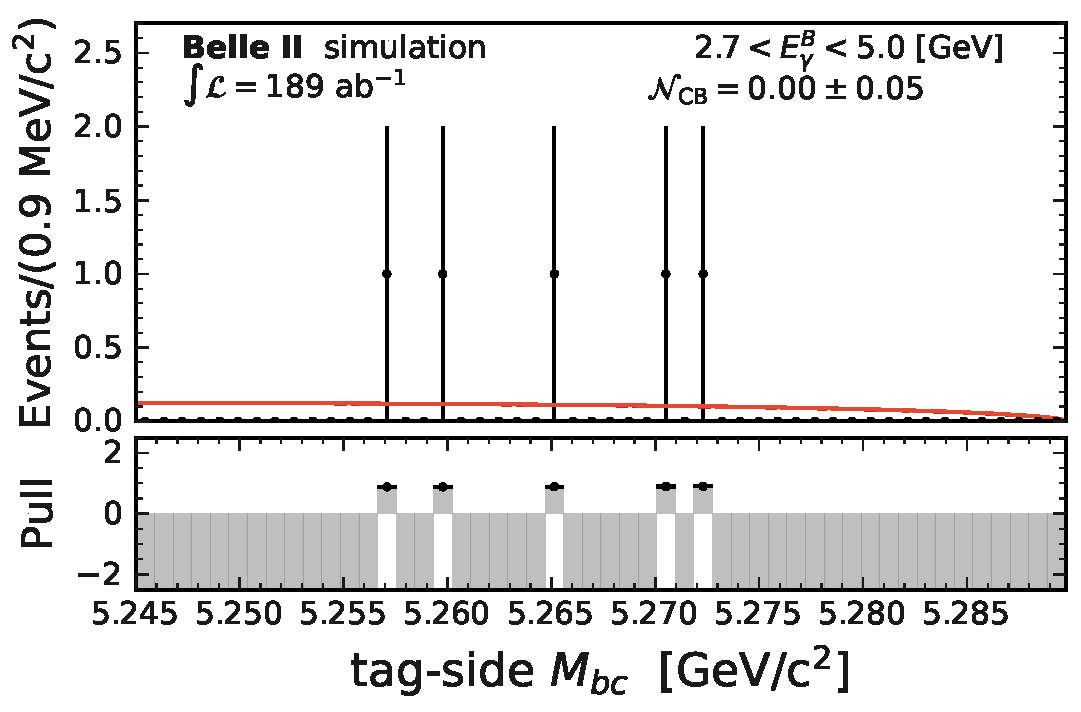
\includegraphics[width=0.3\textwidth]{figures/data_validation/bbbar_enhanced_fits/MC_MbcFit_2p7to5p0ppdf.pdf}
    }
    \caption{\label{fig:mbc_bbar_ehnhanced_fits_mc}
    The fits on Belle II simulation corresponding to 1.6~\invfb with selection 
    that enhances non-\BtoXsgamma events, as discussed in \Cref{sec:continuum_spectrum_validation}.
    The fitting model from \Cref{tab:fitting_init_params_updated} is used,
    which is defined on the `corrected'-\Mbc to account for variations $\sqrt{s}$ in Belle II data.
    Good description of the \Mbc distributions can be seen throughout the \EB bins.
    }
\end{figure}
\begin{figure}[htbp!]
    \centering
    \subcaptionbox{\label{fig:mbc_bbar_ehnhanced_data_1p4}}{
        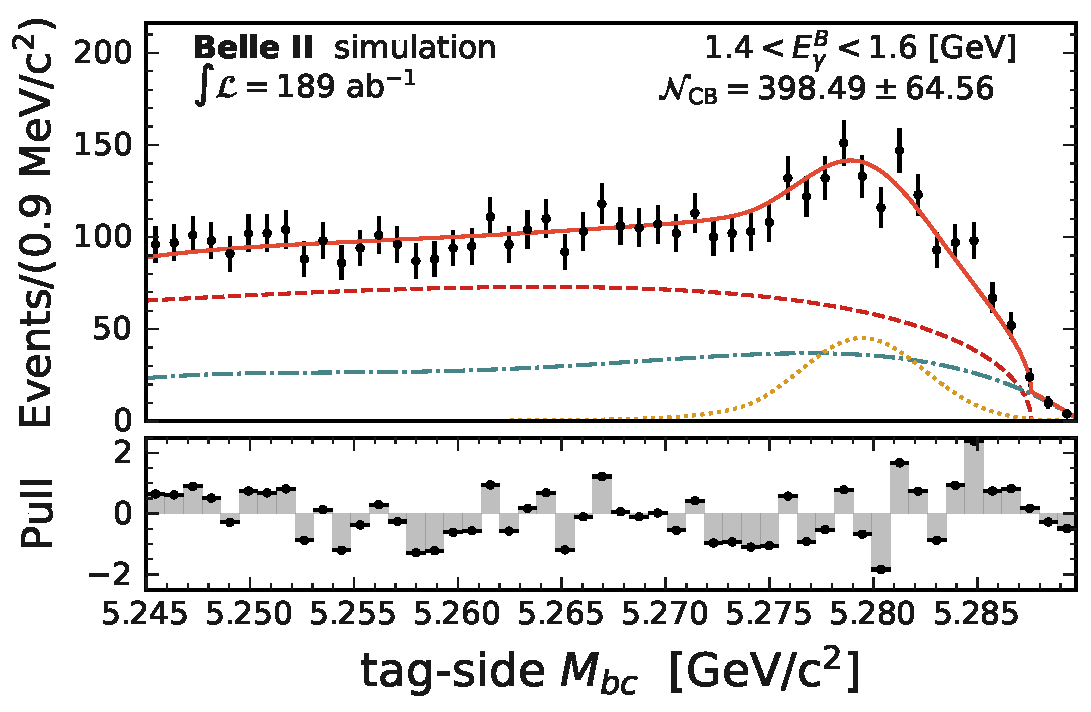
\includegraphics[width=0.3\textwidth]{figures/data_validation/bbbar_enhanced_fits/DATA_MbcFit_1p4to1p6ppdf.pdf}
    }
    \subcaptionbox{\label{fig:mbc_bbar_ehnhanced_data_1p6}}{
        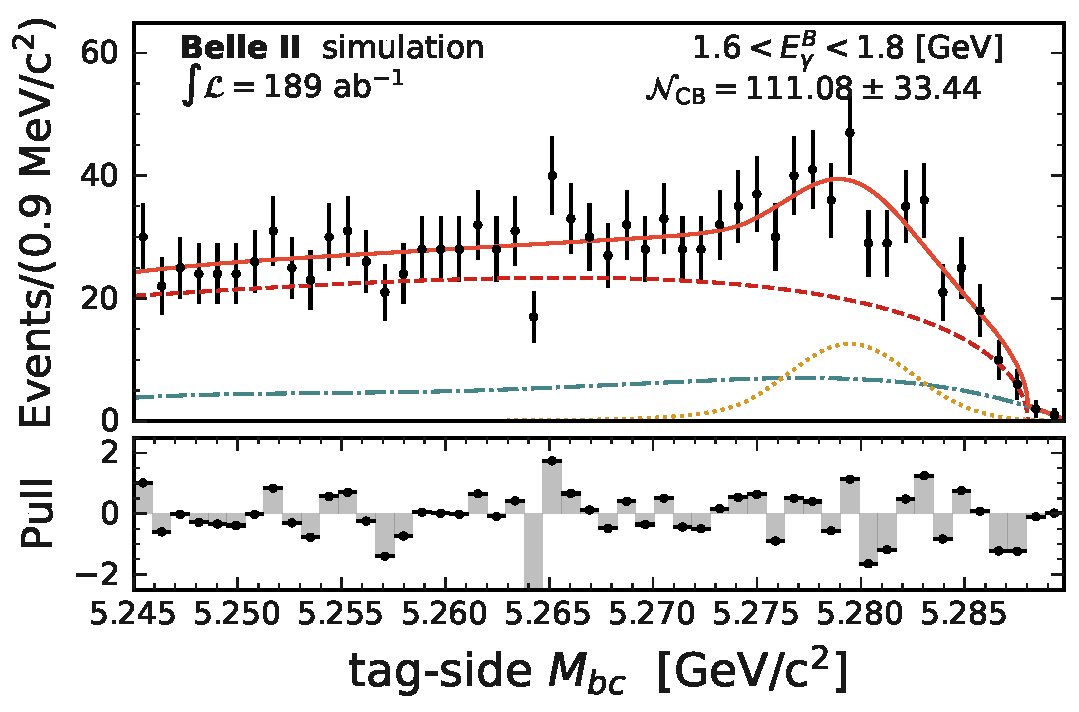
\includegraphics[width=0.3\textwidth]{figures/data_validation/bbbar_enhanced_fits/DATA_MbcFit_1p6to1p8ppdf.pdf}
    }
    \subcaptionbox{\label{fig:mbc_bbar_ehnhanced_data_1p8}}{
        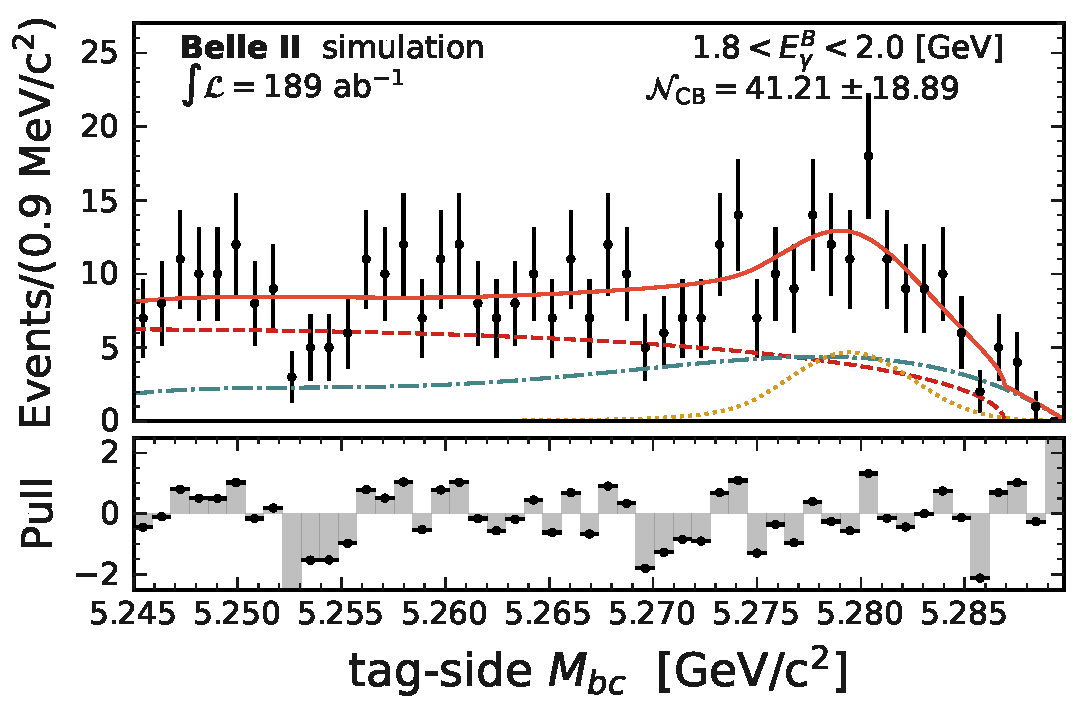
\includegraphics[width=0.3\textwidth]{figures/data_validation/bbbar_enhanced_fits/DATA_MbcFit_1p8to2p0ppdf.pdf}
    }
    \subcaptionbox{\label{fig:mbc_bbar_ehnhanced_data_2p0}}{
        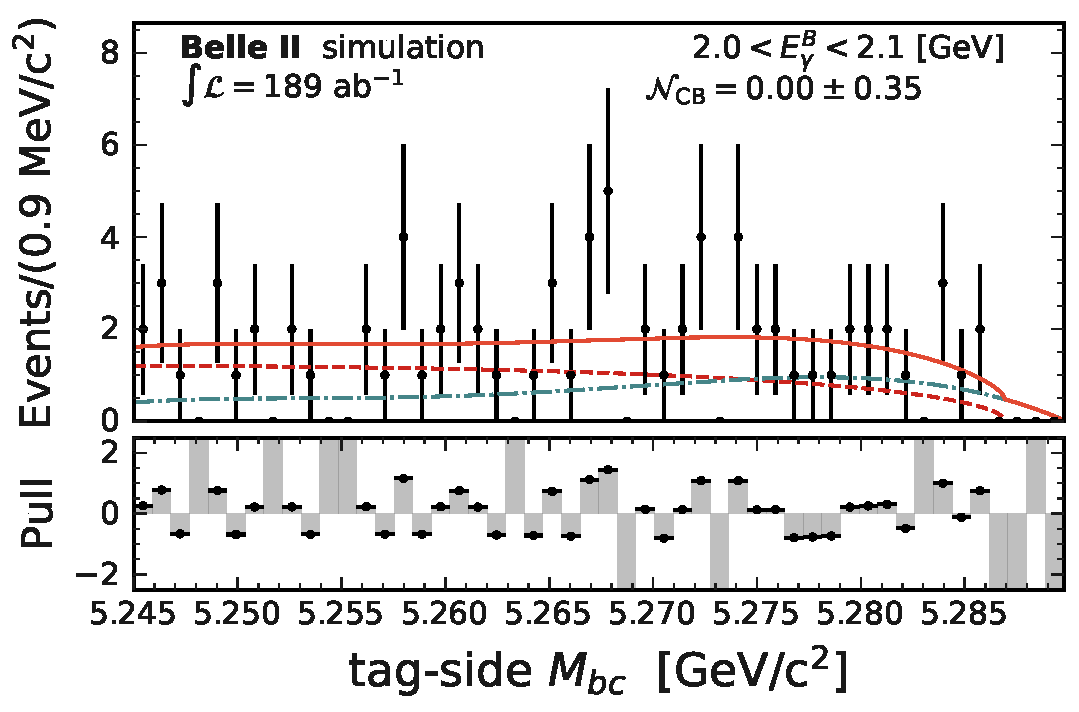
\includegraphics[width=0.3\textwidth]{figures/data_validation/bbbar_enhanced_fits/DATA_MbcFit_2p0to2p1ppdf.pdf}
    }
    \subcaptionbox{\label{fig:mbc_bbar_ehnhanced_data_2p1}}{
        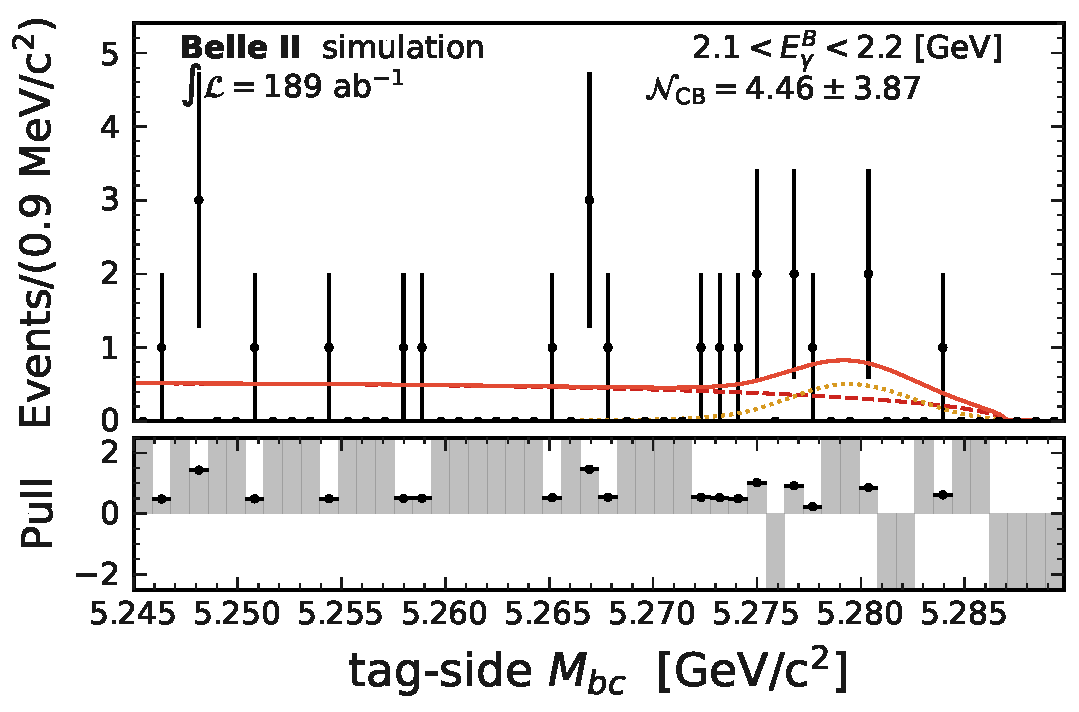
\includegraphics[width=0.3\textwidth]{figures/data_validation/bbbar_enhanced_fits/DATA_MbcFit_2p1to2p2ppdf.pdf}
    }
    \subcaptionbox{\label{fig:mbc_bbar_ehnhanced_data_2p2}}{
        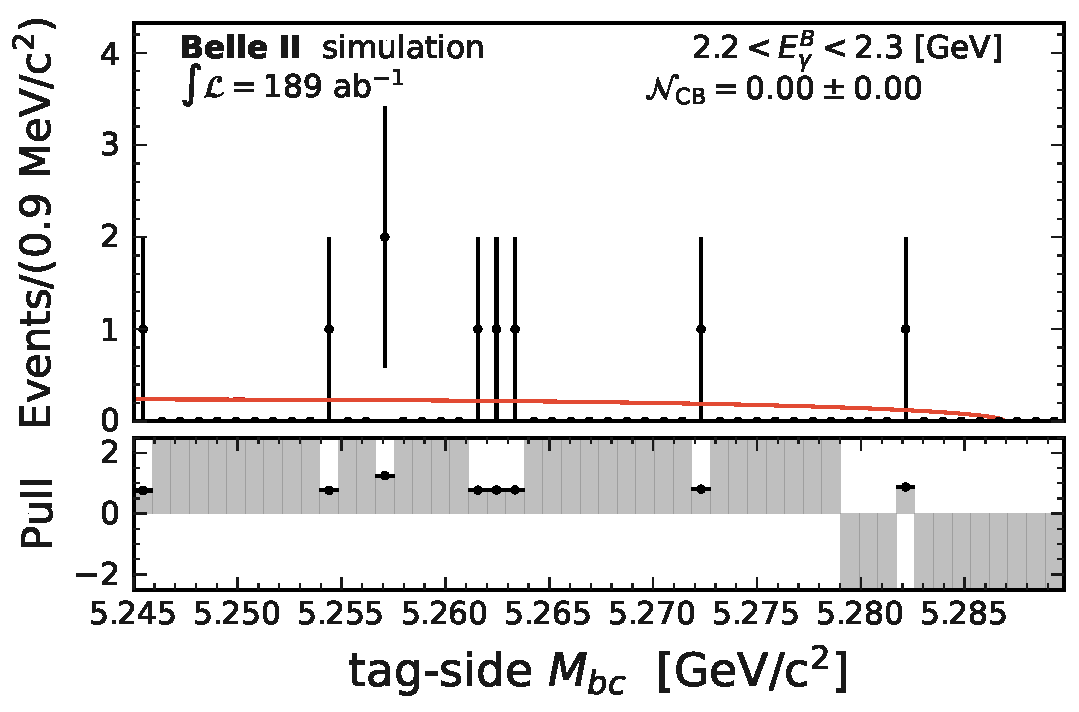
\includegraphics[width=0.3\textwidth]{figures/data_validation/bbbar_enhanced_fits/DATA_MbcFit_2p2to2p3ppdf.pdf}
    }
    \subcaptionbox{\label{fig:mbc_bbar_ehnhanced_data_2p3}}{
        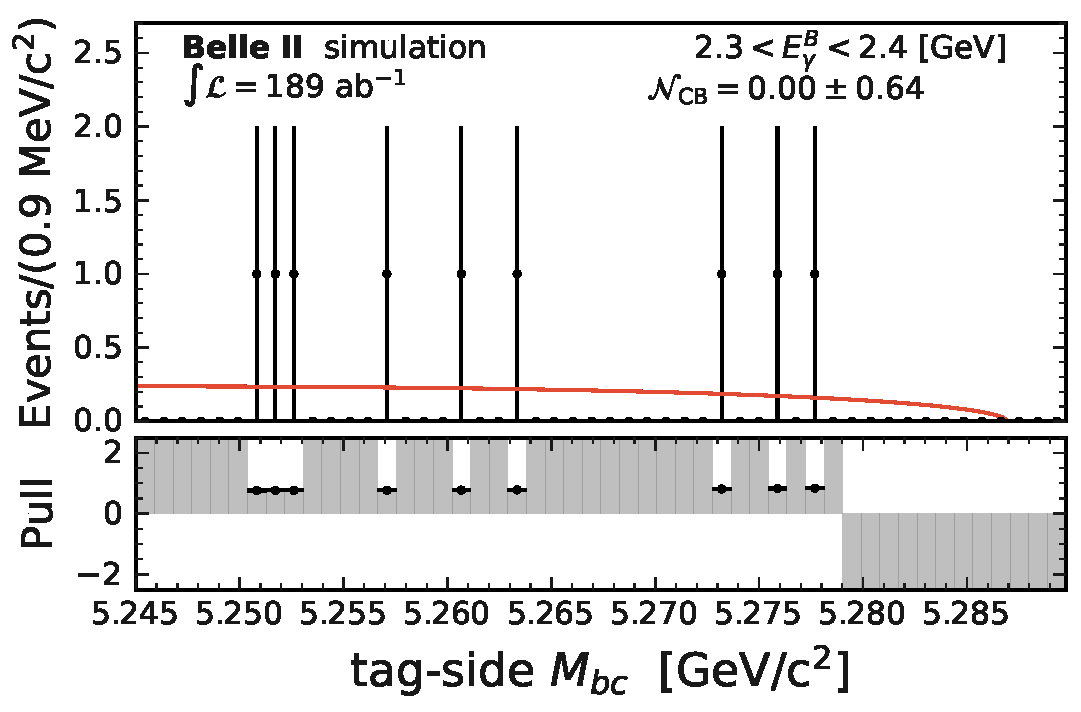
\includegraphics[width=0.3\textwidth]{figures/data_validation/bbbar_enhanced_fits/DATA_MbcFit_2p3to2p4ppdf.pdf}
    }
    \subcaptionbox{\label{fig:mbc_bbar_ehnhanced_data_2p4}}{
        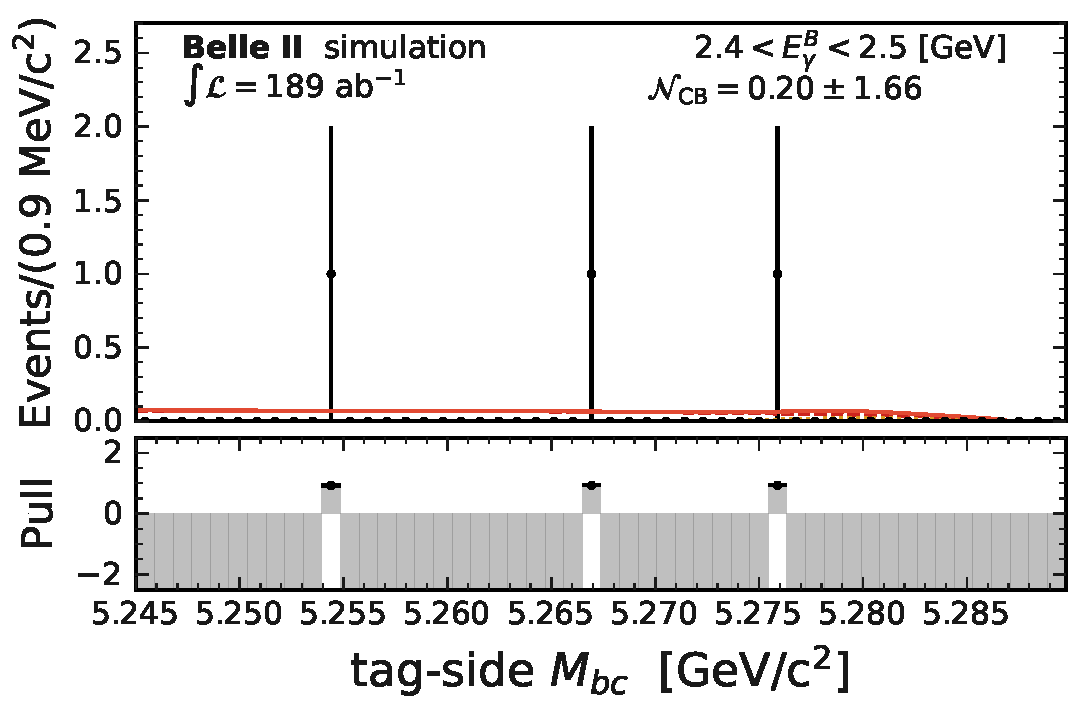
\includegraphics[width=0.3\textwidth]{figures/data_validation/bbbar_enhanced_fits/DATA_MbcFit_2p4to2p5ppdf.pdf}
    }
    \subcaptionbox{\label{fig:mbc_bbar_ehnhanced_data_2p5}}{
        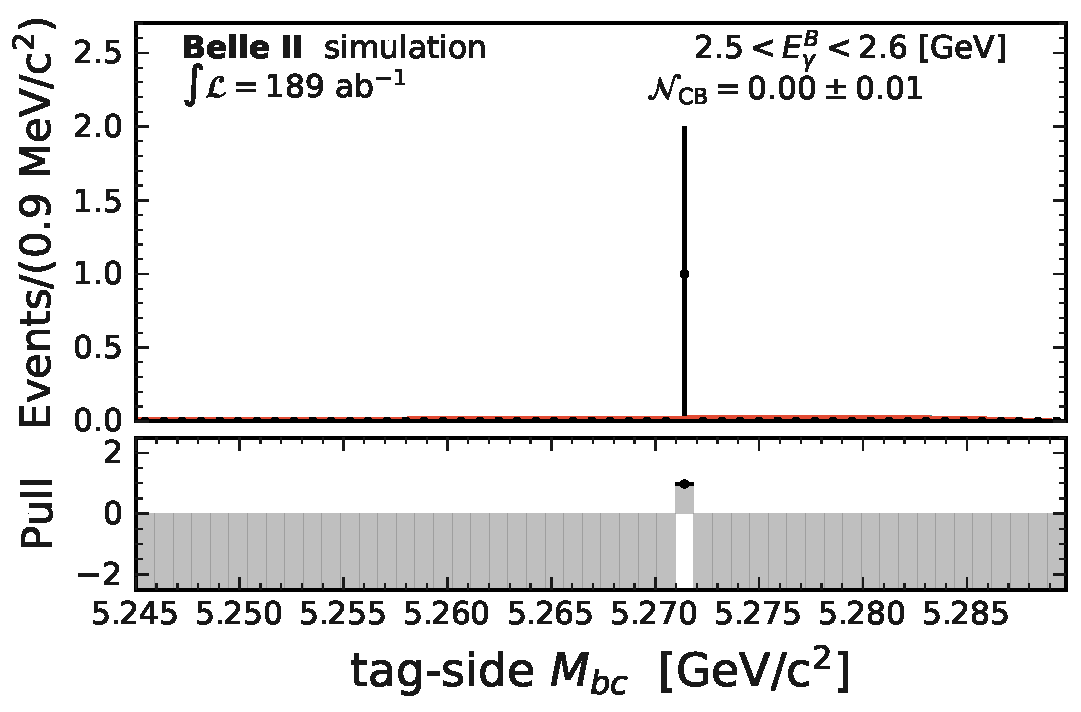
\includegraphics[width=0.3\textwidth]{figures/data_validation/bbbar_enhanced_fits/DATA_MbcFit_2p5to2p6ppdf.pdf}
    }
    \subcaptionbox{\label{fig:mbc_bbar_ehnhanced_data_2p6}}{
        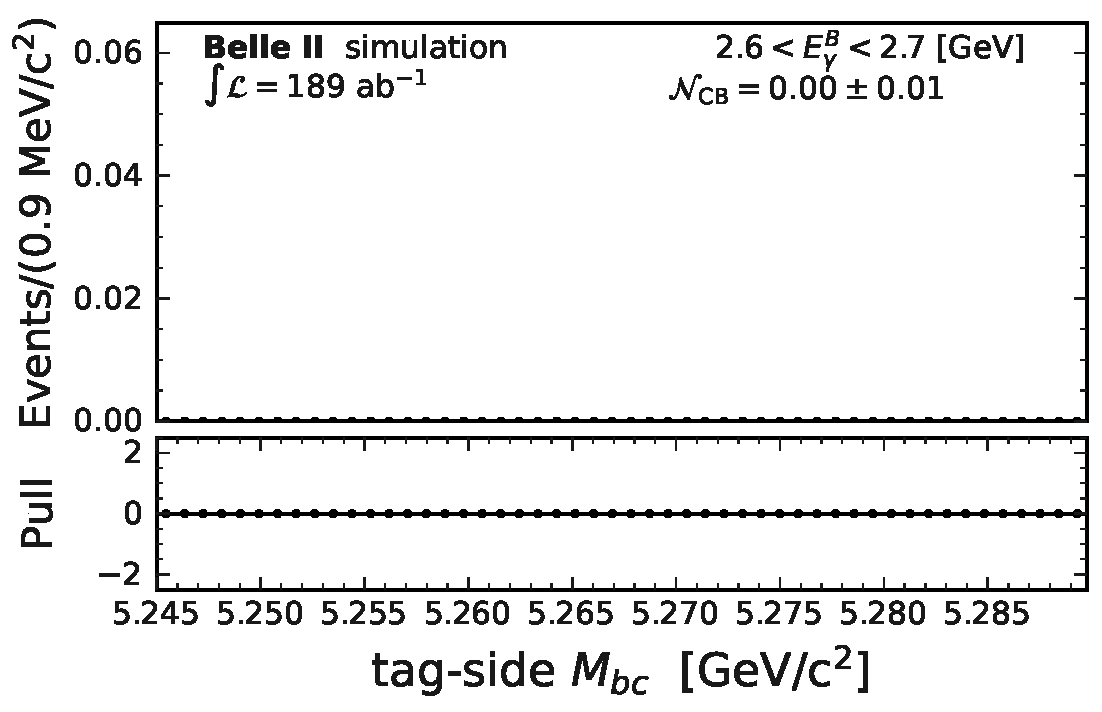
\includegraphics[width=0.3\textwidth]{figures/data_validation/bbbar_enhanced_fits/DATA_MbcFit_2p6to2p7ppdf.pdf}
    }
    \subcaptionbox{\label{fig:mbc_bbar_ehnhanced_data_2p7}}{
        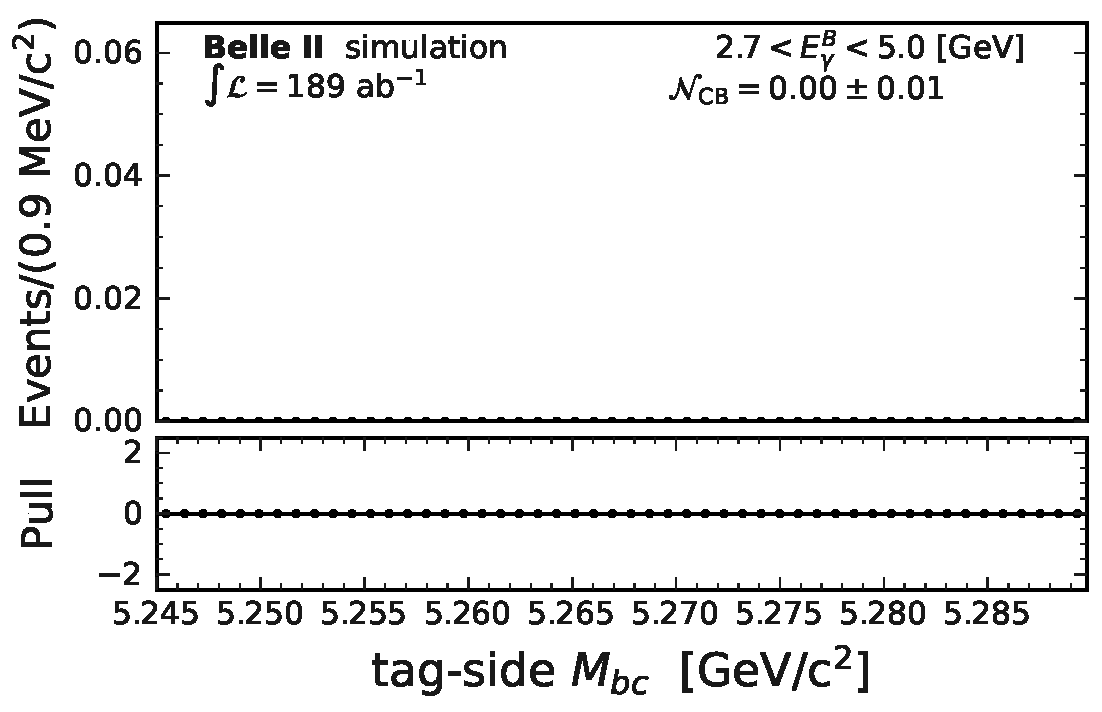
\includegraphics[width=0.3\textwidth]{figures/data_validation/bbbar_enhanced_fits/DATA_MbcFit_2p7to5p0ppdf.pdf}
    }
    \caption{\label{fig:mbc_bbar_ehnhanced_fits_data}
    The fits on Belle II data corresponding to 189~\invfb with selection 
    that enhances non-\BtoXsgamma events, as discussed in \Cref{sec:continuum_spectrum_validation}.
    The fitting model from \Cref{tab:fitting_init_params_updated} is used,
    which is defined on the `corrected'-\Mbc to account for variations $\sqrt{s}$ in Belle II data.
    Good description of the \Mbc distributions can be seen throughout the \EB bins.
    }
\end{figure}

Despite a vastly varying number of events and shapes of the total distribution throughout different \EB intervals,
the fitter performs well.
The extracted $\mathcal{N}_{\mathrm{CB}}^{\mathrm{DATA}}$ $\mathcal{N}_{\mathrm{CB}}^{\mathrm{MC}}$ (corresponding to good tag-\B meson yields in data and simulation, respectively)
are directly compared.
Correcting the simulation based on \Cref{tab:correction_table} (with inverted \piVeto and \etaVeto correction as shown in \Cref{eq:correction_transform}) and calculating the difference between the two is expected to yield a value consistent with zero.
The resulting difference, with appropriate statistical uncertainties and uncertainties from corrections applied are shown in \Cref{fig:bbar_enhanced_background_subtraction}.
The hypothesised result is observed, confirming the adequacy of the fitter, the validity of background-subtraction procedure and the corrections, that were applied.

\begin{figure}[htbp!]
    \centering
    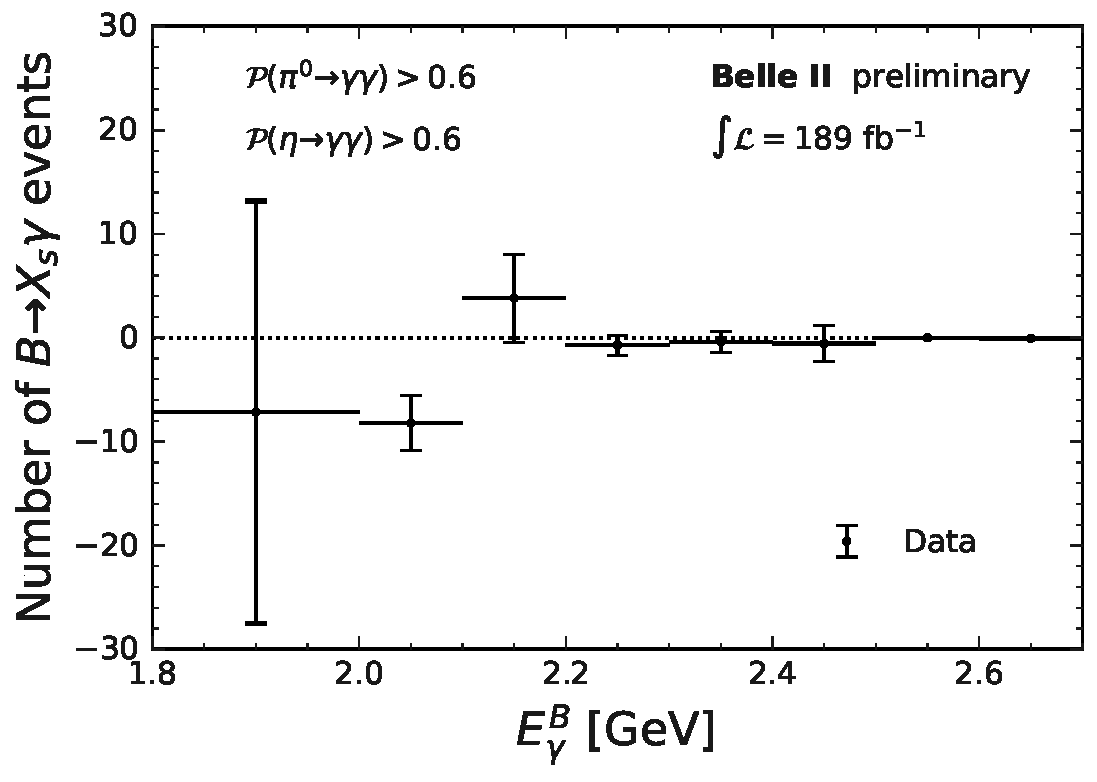
\includegraphics[width=0.45\textwidth]{figures/data_validation/bbar_enhanced_event_counts.pdf}
    \caption{\label{fig:bbar_enhanced_background_subtraction}
    The number of events after subtracting good tag-\B meson counts extracted from fits in Belle~II simulation (\Cref{fig:mbc_bbar_ehnhanced_fits_mc}),
    from that in Belle~II data (\Cref{fig:mbc_bbar_ehnhanced_fits_data}).
    The simulated values are corrected for luminosity and to better represent data based on studies in \Cref{sec:corrections}.
    The background subtraction procedure is further detailed in \Cref{sec:background_subtraction,sec:background_subtraction_validation_mc}.
    Here, an agreement with 0 is expected in all \EB bins (no \BtoXsgamma events are present).
    }
\end{figure}

\subsection{Validation outside of the \texorpdfstring{\EB}{EB} signal-region}\label{sec:sidebands_validation}

In \Cref{sec:continuum_spectrum_validation,sec:continuum_mbc_validation,sec:bb_background_validation} it was seen that the background simulation of \qqbar and \BB events,
althought not perfect, is described adequatly by the \Mbc fitter yielding correct and valid estimation of good tag-\B mesons in data and simulation.
The last validation performed for background simulation is done outside of \EB signal region.
As discussed in \Cref{sec:binning}, the $\EB\in(1.4-1.8)~\gev$ and $2.7<\EB~\gev$ intervals were selected as sideband regions, 
due to a small number of \BtoXsgamma events and a low signal-to-background ratio expected there.
The same argumentation make the regions excellent for background validation.

The \EB distribution, for the three \EB sideband intervals are shown in \Cref{fig:sidebands_eb}.
A striking, nearly 20\%, difference in normalisation is observed, 
which seems similar to that observed in \Cref{fig:qqbar_enhanced_eb_validation}.
Interestingly, here, the \epem\ra\qqbar component is thought to be strongly suppressed by \texttt{BDT~output}.
To better understand this discrepancy, the corrected-\Mbc distributions in each \EB sideband bin are inspected.
This is shown in \Cref{fig:sidebands_mbc}.
\begin{figure}[htbp!]
    \centering
    \subcaptionbox{\label{fig:Bplus_sidebands_eb}}{
        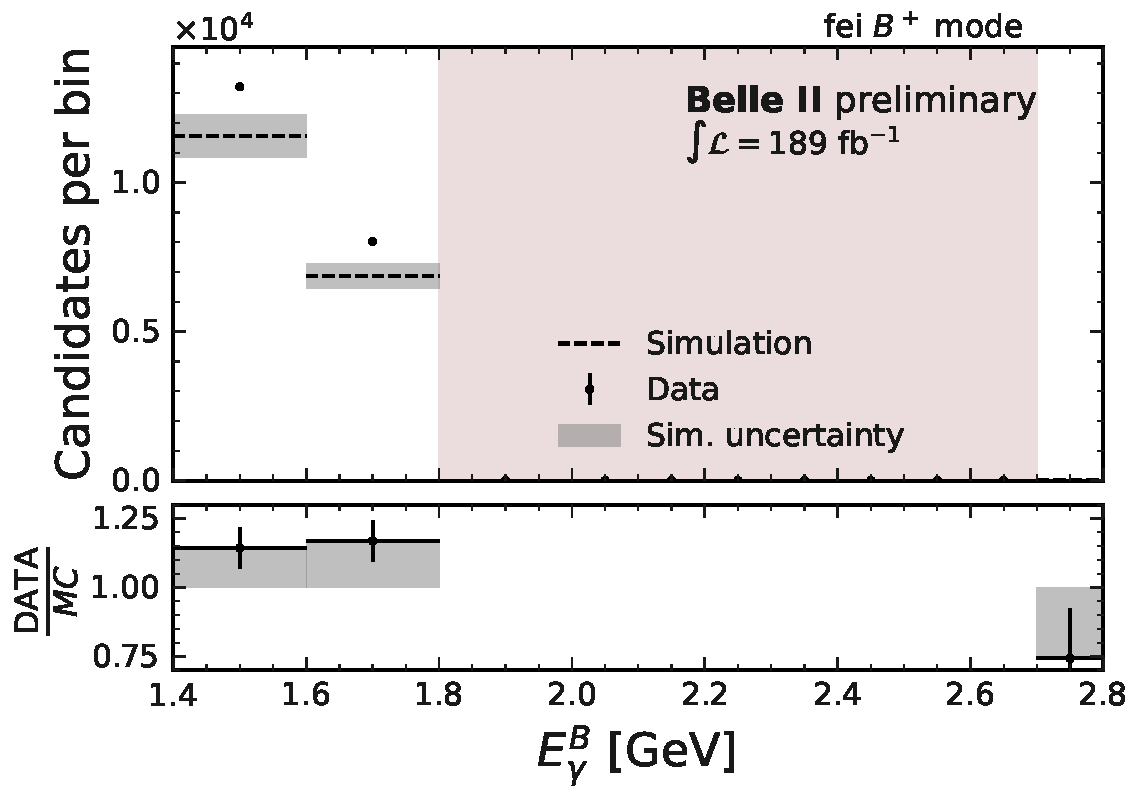
\includegraphics[width=0.31\textwidth]{figures/data_validation/Bplus_sidebands_eb.pdf}
    }
    \subcaptionbox{\label{fig:Bzero_sidebands_eb}}{
        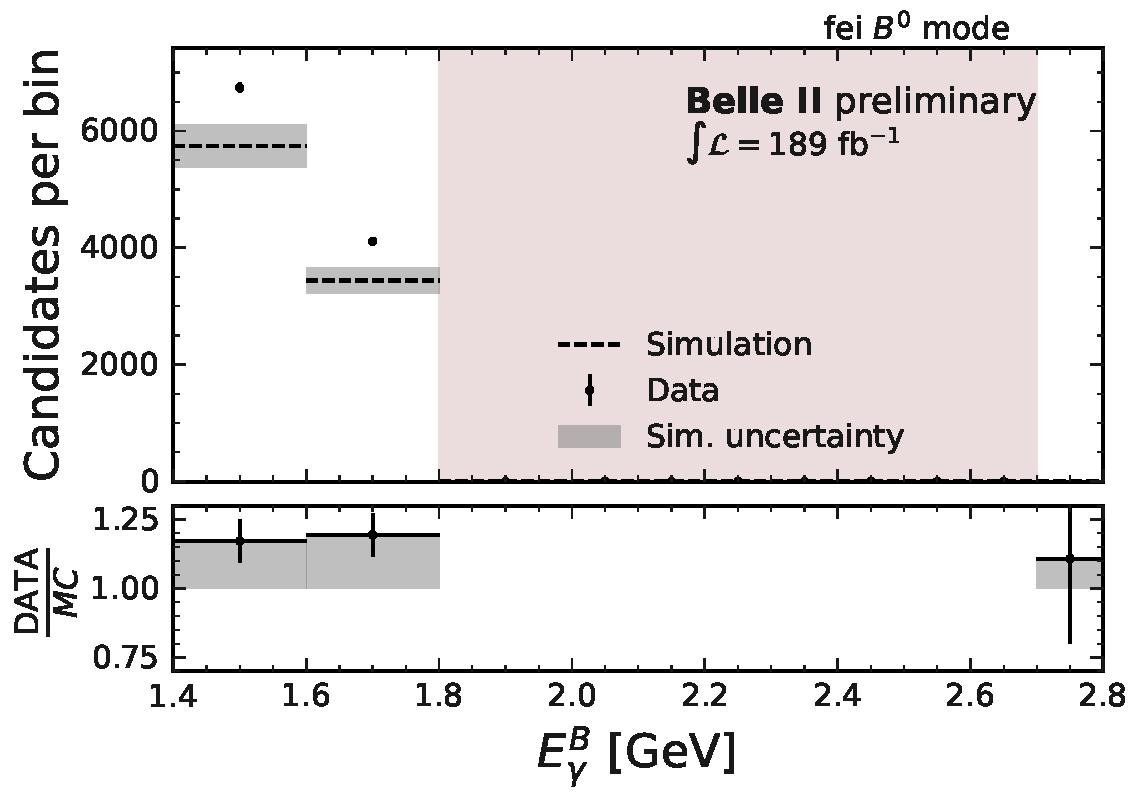
\includegraphics[width=0.31\textwidth]{figures/data_validation/Bzero_sidebands_eb.pdf}
    }
    \subcaptionbox{\label{fig:Bboth_sidebands_eb}}{
        \includegraphics[width=0.31\textwidth]{figures/data_validation/Bboth_sidebands_eb.pdf}
    }
    \caption{\label{fig:sidebands_eb} 
    The \EB distribution of the \EB sideband regions (see \Cref{sec:sidebands_validation}).
    The low-\EB region side sees a roughly 20\% discrepancy.
    The shaded area represents the signal region which is blinded: during the validation step it was not observed.
    }
\end{figure}
\begin{figure}[htbp!]
    \centering
    \subcaptionbox{\label{fig:sidebands_mbc1}}{
        \includegraphics[width=0.31\textwidth]{figures/data_validation/sidebands_mbc_1.pdf}
    }
    \subcaptionbox{\label{fig:sidebands_mbc2}}{
        \includegraphics[width=0.31\textwidth]{figures/data_validation/sidebands_mbc_2.pdf}
    }
    \subcaptionbox{\label{fig:sidebands_mbc3}}{
        \includegraphics[width=0.3\textwidth]{figures/data_validation/sidebands_mbc_3.pdf}
    }1
    \caption{\label{fig:sidebands_mbc} 
    The \Mbc distribution of the \EB sideband regions (see \Cref{sec:sidebands_validation}).
    The figures showcase different \EB ranges, as indicated on the right corner of each Figure.
    Interestingly, a similar low-\Mbc discrepancy is observer as that with the enhanced-continuum sample, shown in \Cref{fig:qqbar_enhanced_mbc}.
    }
\end{figure}

The results of \Cref{fig:sidebands_eb,fig:sidebands_mbc} indicate that Belle~II data, especially the low-\Mbc region, has a clear excess compared to simulation.
While some discrepancy is expected considering the results of \Cref{fig:qqbar_enhanced_mbccorrected},
the larger scale of the discrepancy is confusing -- given the fact that this was not observed in \Cref{fig:bbbar_enhanced_mbccorrected}.
Although more studies on this subject are necessary to fully understand the discrepancy, 
it is attributed to a \BB-background component which is not well modelled in Belle~II simulation, the potential origin of which is shortly discussed here.
\todo[inline]{add see discussion here XX}

In particular, consider the removal of \texttt{zernikeMVA} selection.
The resulting \EB sideband distribution and the \Mbc distribution are shown in \Cref{fig:nozmva_test}.
In this case, the agreement between data and simulation in the \EB-sideband spectrum appears to be near-perfect.
Indeed, even considering the \Mbc distribution for $\EB\in(1.4,1.6)~\gev$, one clearly observes a better overall-agreement.
These observations strongly suppor the previous hypothesis that a hadronic cluster is not well-modelled in simulation.
The component cannot be common to \epem\ra\qqbar events, because the effect was not seen in off-resonance data in \Cref{sec:continuum_spectrum_validation}.
As a result, this component is suppressed in Belle~II simulation by a selection on the \texttt{zernikeMVA} observable, but this does happen in Belle~II data.
\begin{figure}[htbp!]
    \subcaptionbox{\label{fig:sideband_eb_nozmva}}{
        \includegraphics[width=0.31\textwidth]{figures/data_validation/Bboth_sidebands_eb_nozmva.pdf}
    }
    \subcaptionbox{\label{fig:sideband_mbc_nozmva}}{
        \includegraphics[width=0.31\textwidth]{figures/data_validation/sidebands_mbc_nozmva_1.pdf}
    }
    \subcaptionbox{\label{fig:zmva_discrepancy}}{
        \includegraphics[width=0.31\textwidth]{figures/data_validation/Bboth_sidebands_zmva.pdf}
    }
    \caption{\label{fig:nozmva_test}   The \EB distributions in the \EB sideband region (\Cref{fig:sideband_eb_nozmva})
    and the \Mbc distribution in $1.4<\EB<1.6~\gev$ regions in both cases the optimised requirement on $\mathtt{zernikeMVA}$.
    \Cref{fig:zmva_discrepancy} is the full-range of the \ZMVA distribution.
    The \Cref{fig:sideband_eb_nozmva,fig:sideband_mbc_nozmva} can be directly compared with \Cref{fig:Bboth_sidebands_eb,fig:sidebands_mbc3}, respectively.
    Without the $\mathtt{zernikeMVA}$ the agreement between data and simulation appears to be improved indicating that a component in data is not simulated adequatly.
    The presence of a mismodelled component in Belle~II simulation is apparent when inspecting the \ZMVA distribution.
    }
\end{figure}

These considerations are supported by inspecting the \ZMVA distribution in the $\mbox{\EB\in(1.4,1.8)~\gev}$ region, as seen in \Cref{fig:zmva_discrepancy}.
While simulation contains a sharp peak near 0, this is not evident in Belle~II data, which on the other hand has an excess at high-\ZMVA.
Hence, the background-suppression efficiency is not well-represented in simulation.
These results are also conflated with the differences in \Mbc endpoint, making an exact evaluation of the effect difficult at this stage.
Independent studies of the \ZMVA distributions, performed similarly to the photon detection efficiency study described in \Cref{sec:photon_efficiency}, did not observe the presence of such peak.
This may imply that this type of selection is particular for photon candidates from \BB events misidentified as high-energy photons.
Therefore, it was concluded that additional studies of \ZMVA in the context of radiative and inclusive analyses will be necessary for future iterations of this analysis.

While these observations are alarming, so far all the results have shown that the \Mbc fitter and background-subtraction procedure were robust against the
continuum \Mbc distribution shape differences, as seen in \Cref{sec:continuum_mbc_validation,sec:bb_background_validation}.
Therefore, the further analysis does not replace or remove the \ZMVA requirement.

The fit is performed on the full sample of data, however, the results from the signal region, $\EB\in(1.8,2.7)$ are hidden and not investigated at this stage.
The individual \Mbc fits on the \EB sideband regions are shown for data in \Cref{fig:sideband_data_fit}, and for simulation in \Cref{fig:sideband_mc_fit}.
\begin{figure}[htbp!]
    \centering
    \subcaptionbox{\label{fig:sideband_data_fit_1}}{
        \includegraphics[width=0.31\textwidth]{figures/data_validation/sidebands_fit/DATA_MbcFit_1p4to1p6ppdf.pdf}
    }
    \subcaptionbox{\label{fig:sideband_data_fit_2}}{
        \includegraphics[width=0.31\textwidth]{figures/data_validation/sidebands_fit/DATA_MbcFit_1p6to1p8ppdf.pdf}
            }
    \subcaptionbox{\label{fig:sideband_data_fit_11}}{
        \includegraphics[width=0.31\textwidth]{figures/data_validation/sidebands_fit/DATA_MbcFit_2p7to5p0ppdf.pdf}
    }
    \caption{\label{fig:sideband_data_fit}    
    The \Mbc fits on Belle II data corresponding to 189~\invfb of data in \EB sideband regions,
    as discussed in \Cref{sec:sidebands_validation}.
    The fitting model from \Cref{tab:fitting_init_params_updated} is used,
    which is defined on the `corrected'-\Mbc to account for variations $\sqrt{s}$ in Belle II data.
    Good description of the \Mbc distributions can be seen throughout the \EB bins.
    }
\end{figure}
\begin{figure}[htbp!]
    \centering
    \subcaptionbox{\label{fig:sideband_mc_fit_1}}{
        \includegraphics[width=0.31\textwidth]{figures/data_validation/sidebands_fit/NOSIGNALMC_MbcFit_1p4to1p6ppdf.pdf}
    }
    \subcaptionbox{\label{fig:sideband_mc_fit_2}}{
        \includegraphics[width=0.31\textwidth]{figures/data_validation/sidebands_fit/NOSIGNALMC_MbcFit_1p6to1p8ppdf.pdf}
            }
    \subcaptionbox{\label{fig:sideband_mc_fit_3}}{
        \includegraphics[width=0.31\textwidth]{figures/data_validation/sidebands_fit/NOSIGNALMC_MbcFit_2p7to5p0ppdf.pdf}
    }
    \caption{\label{fig:sideband_mc_fit}    
    The \Mbc fits on Belle II simulation corresponding to 189~\invfb of data in \EB sideband regions,
    as discussed in \Cref{sec:sidebands_validation}.
    These distributions contain no \BtoXsgamma events, although even without the requirement the number of radiative transitions in these energy ranges are negligible.
    The fitting model from \Cref{tab:fitting_init_params_updated} is used,
    which is defined on the `corrected'-\Mbc to account for variations $\sqrt{s}$ in Belle II data.
    Good description of the \Mbc distributions can be seen throughout the \EB bins.
    }
\end{figure}

The summarised results of the good tag-\B meson yields estimated in the \Mbc fits are shown in \Cref{fig:sidebands_background_versus_data}.
In the high-\EB sideband no peaking tag-\B mesons are observed in data or simulation, which is exactly consistent with the naive expectations.
In the low-\EB region a large number of events is observed.
Clearly, the data points are compatible with the background expectation, although the estimates in both intervals are higher than the expected background.
Subtracting the background expectation from the good tag-\B meson yield in data results in \Cref{fig:sidebands_subtracted}.
A similar observation follows: although both values are (nearly) compatible with zero,
the central values are slightly positive.

\begin{figure}[htbp!]
    \centering
    \includegraphics[width=0.45\textwidth]{figures/data_validation/sidebands_background_vs_data.pdf}
    \caption{\label{fig:sidebands_background_versus_data} The results of fitting the \Mbc on the sideband region in data (see \Cref{sec:sidebands_validation}).
    The values corresponding to data fits are estimated through an \Mbc fit shown in \Cref{fig:sideband_data_fit}.
    The remaining-\BB background expectations are estimated through \Mbc fits in \Cref{fig:sideband_mc_fit} and \Cref{fig:nosignal_fits_signal}.
    The signal region in this figure is blinded, therefore only simulation results are shown.
    The extracted results from the data fit and simulated background expectations 
    are compatible within their full uncertainty, but both points are higher than the background estimation.
    }
\end{figure}

\begin{figure}[htbp!]
    \centering
    \subcaptionbox{\label{fig:sidebands_subtracted}}{
        \includegraphics[width=0.45\textwidth]{figures/data_validation/sideband_event_counts.pdf}
    }
    \subcaptionbox{\label{fig:sidebands_subtracted_corrected}}{
        \includegraphics[width=0.45\textwidth]{figures/data_validation/sideband_event_counts_corrected.pdf}
    }
    \caption{\label{fig:sidebands_subtracted_figures} The results of subtraction of the remaining-\BB background after the fit on Belle~II data.
    \Cref{fig:sidebands_subtracted} show the results with no correction factor applied.
    \Cref{fig:sidebands_subtracted_corrected} includes an 8.7\% scaling factor for the simulated background values.
    The signal region, denoted by the shaded area, is blinded at this stage.
    In this analysis it is chosen to scale the background (i.e. scenario shown in \Cref{fig:sidebands_subtracted_corrected}),
    as that region is expected to contain a number of \BtoXsgamma events consistent with 0.
    This figure only includes systematic uncertainties related to simulation corrections described in \Cref{sec:corrections}.
    }
\end{figure}

The total number of events in the low-\EB sideband are $2698\pm139$ (expected to be predominantly background, see \Cref{sec:binning}).
The background expectation from simulation in the same region is $2483\pm130$.
Taking the ratio of these values yields $1.087\pm0.080$.
As this value is not compatible with unity within $1\sigma$, a background scaling of 8.7\% is adopted.
100\% of the scaling will also be adopted as a systematic uncertainty later.
The scaled-background-subtracted data fit yields are shown in \Cref{fig:sidebands_subtracted_corrected}.
By construction, they are fully compatible with zero.

% \subsection{Summary of study of validation samples}\label{sec:summary_of_validation}

% As there was quite a few important points presented in \Cref{sec:validation}, 
% a quick summary is produced here to condense the most important findings.
% The main observations are as follows:
% \begin{itemize}
%     \item Good \EB spectrum description in \epem\ra\qqbar events, is observed in \Cref{sec:continuum_spectrum_validation,sec:continuum_mbc_validation}.
%     \item Problems with \Mbc distribution endpoint modelling, related to experimental condition variations in Belle~II data, which are not captured in run-period-independent simulation.
%     This is observed in \Cref{sec:continuum_mbc_validation}.
%     \item Related to the last point, differences with the shape of \epem\ra\qqbar events in simulation and data.
%     \item A new, corrected \Mbc variable introduced to partially compensate the \Mbc endpoint difference in data and simulation.
%     \item The fitter is able to accurately describe the number of good tag-\B meson events in data and simulation.
%     \item A scaling factor is introduced, which will also be adopted as a systematic uncertainty related to normalisation.
% \end{itemize}




